% =====================================================================
%  Manuscript for MDPI *Electronics* (official LaTeX template).
%
%  HOW TO COMPILE (this file targets the official MDPI class):
%   1. Get the MDPI LaTeX template:
%        - Overleaf: New Project -> Templates -> search "MDPI" (journal: Electronics), OR
%        - https://www.mdpi.com/authors/latex  (download the LaTeX zip).
%   2. Drop THIS main.tex and refs.bib into the template folder
%      (which provides Definitions/mdpi.cls, the logos and *.bst).
%   3. Put the figures from paper/figures/*.png next to main.tex (or keep the path).
%   4. Build order:  pdflatex -> bibtex -> pdflatex -> pdflatex
%
%  All numbers below come from the reproducible experiments in this repo
%  (phase1/, phase2/, paper/experiments/secom_validation.py).
% =====================================================================
\documentclass[electronics,article,submit,pdftex,moreauthors]{Definitions/mdpi}

% --- If the MDPI class is unavailable and you only want to preview the text,
% --- comment the line above and uncomment the minimal fallback below:
% \documentclass[11pt]{article}
% \usepackage{graphicx,booktabs,amsmath,amssymb,hyperref,authblk,geometry,tabularx}
% \geometry{a4paper,margin=2.3cm}\graphicspath{{figures/}}

\graphicspath{{figures/}{paper/figures/}}

% Official MDPI bibliography workflow (BibTeX + Definitions/mdpi.bst from the template)
\externalbibliography{yes}

\Title{Knowledge-Graph-Guided Detection of Hidden Multi-Parameter Failures and Core-Indicator Selection for Retired-Chip Remanufacturing}

\TitleCitation{Knowledge-Graph-Guided Detection of Hidden Multi-Parameter Failures and Core-Indicator Selection for Retired-Chip Remanufacturing}

\Author{First Author $^{1,\dagger}$, Second Author $^{2}$ and Corresponding Author $^{1,*}$}

\AuthorNames{First Author, Second Author and Corresponding Author}

\address{%
$^{1}$ \quad Affiliation 1, City, Country; email1@example.com\\
$^{2}$ \quad Affiliation 2, City, Country; email2@example.com}

\corres{Correspondence: corresponding@example.com}

\abstract{The reuse and remanufacturing of retired integrated-circuit (IC) chips is a key lever for a circular electronics economy, yet conventional pass/fail screening evaluates each test indicator independently and therefore misses \emph{hidden failures}---chips on which every individual indicator is within specification but whose joint combination is unreliable. We present a knowledge-graph-guided framework that (i) organizes multi-dimensional chip test data (physical, DC-electrical, AC-electrical and aging indicators) into a relational knowledge graph with TransE embeddings, (ii) optimizes indicator features and identifies failures with a hybrid graph neural network (GCN+GAT) and gradient-boosted trees, and (iii) quantifies each indicator's marginal contribution with Shapley (SHAP) values to compress the test suite to a small core set. On a controlled synthetic benchmark of 1000 chips---purpose-built so that failures arise from non-convex \emph{combinations} of individually in-specification indicators---a linear model reaches only 0.845 AUC, whereas a nonlinear classifier on optimized features attains 0.961 AUC and 0.940 accuracy (5-fold out-of-fold), confirming that multi-indicator nonlinear interaction, not any single threshold, governs the hidden failures. SHAP-based selection reduces 28 indicators to 6 while retaining 95\% of the full-suite AUC. To address the synthetic-data limitation, we externally validate the methodology on the real-world UCI SECOM semiconductor dataset (1567 wafers, 590 measurements, 14:1 imbalance), where SHAP-guided selection of the top 25 features \emph{improves} AUC from 0.687 to 0.811. The results indicate that the framework provides an interpretable, test-cost-reducing decision aid for chip remanufacturing screening. All data, code and figures are released for reproducibility.}

\keyword{chip remanufacturing; circular economy; knowledge graph; graph neural network; SHAP; feature selection; hidden failure; semiconductor testing; reliability}

\begin{document}

% =====================================================================
\section{Introduction}
% =====================================================================
Waste electrical and electronic equipment (WEEE) is among the fastest-growing waste streams worldwide, and extending the service life of electronic components through reuse, refurbishment and remanufacturing is a central pillar of the circular economy~\cite{deoliveiraneto2023weee}. Within this stream, retired data-center and server hardware is particularly attractive for value recovery: it is decommissioned in large, homogeneous batches, is comparatively well documented, and contains many integrated-circuit (IC) chips that remain electrically functional at end of service. Recovering and re-qualifying such chips simultaneously diverts hazardous waste from landfill and reduces demand for newly fabricated silicon, whose production is energy- and resource-intensive. The economic and environmental case for chip-level reuse is therefore strong; the technical bottleneck is \emph{trustworthy screening}---deciding, reliably and at acceptable cost, which salvaged chips can be safely redeployed.

Industrial chip screening applies a fixed battery of tests spanning several physical domains: visual and dimensional inspection of the package and pins, direct-current (DC) electrical parameters, alternating-current (AC)/timing parameters, functional vectors, and accelerated aging (burn-in). In current practice each measured indicator is compared against an independent specification limit, and a chip is accepted when no single indicator is out of range. This per-indicator decision logic is simple and auditable, but it has a fundamental blind spot: it cannot capture \emph{hidden failures}. A hidden failure is a chip on which \emph{every} indicator is individually within specification, yet whose particular \emph{combination} of near-limit values produces an unreliable device. Classic mechanisms include a compressed logic noise margin formed jointly by output-high (VOH), output-low (VOL) and input-threshold (VIH/VIL) voltages that are each only marginally adverse; a timing margin that collapses only when a tight setup time coincides with a high operating frequency; and a thermal--power spiral in which elevated dynamic current, package warpage and leakage reinforce one another under aging stress. In all of these, no single indicator looks abnormal, but the joint configuration is fatal. Detecting hidden failures therefore requires modeling the joint, generally nonlinear, structure of many indicators at once rather than thresholding indicators one at a time.

Three technical capabilities are needed to do this well. First, a representation that captures the heterogeneous relations among chips, indicators, test stages and failure modes; knowledge graphs are a natural fit and admit embedding methods that surface latent associations~\cite{bordes2013translating,ji2022survey}. Second, a model class able to learn nonlinear interactions among indicators, for which graph neural networks~\cite{kipf2017semi,velickovic2018graph,wu2021comprehensive} and gradient-boosted decision trees~\cite{friedman2001greedy,chen2016xgboost} are leading candidates. Third, interpretability: a remanufacturing line must understand \emph{why} a chip is flagged and which measurements truly matter, both for engineering trust and for reducing test cost. Shapley-value attribution~\cite{shapley1953value,lundberg2017unified,lundberg2020local} provides a principled, model-agnostic answer.

In this paper we integrate these capabilities into a single framework for retired-chip screening and validate it carefully. Our contributions are fourfold:
\begin{itemize}
\item \textbf{A knowledge-graph representation of chip test data.} We model chips, indicators, indicator dimensions, test stages, failure modes and chip models as a typed knowledge graph with data-driven association and abnormality edges, and learn TransE embeddings over it (Section~\ref{sec:kg}).
\item \textbf{A hidden-failure-aware detection pipeline.} We combine domain feature optimization, a hybrid GCN+GAT encoder and gradient-boosted trees to identify failures driven by multi-indicator interaction, benchmarked against a linear, per-indicator reference (Section~\ref{sec:fe}).
\item \textbf{Interpretable core-indicator selection.} Using SHAP values we rank indicator contributions and compress 28 indicators to a 6-indicator core that preserves the bulk of the discriminative power, directly lowering screening cost (Section~\ref{sec:shap}).
\item \textbf{A controlled benchmark plus real-data validation.} We construct a synthetic benchmark in which failures are, by design, non-convex combinations of in-specification indicators, and we externally validate the methodology on the real UCI SECOM semiconductor dataset~\cite{mccann2008secom} (Sections~\ref{sec:data},~\ref{sec:results}).
\end{itemize}

A guiding empirical finding, established quantitatively in Section~\ref{sec:results}, is that on data with genuine hidden-failure structure a \emph{linear} combination of indicators is insufficient while nonlinear models that exploit indicator interactions recover the failures. This directly motivates the graph- and tree-based components of the framework and provides quantitative support for the long-standing intuition that chip re-qualification should be modeled jointly across indicators. The overall pipeline is summarized in Figure~\ref{fig:framework}.

\begin{figure}[H]
\centering
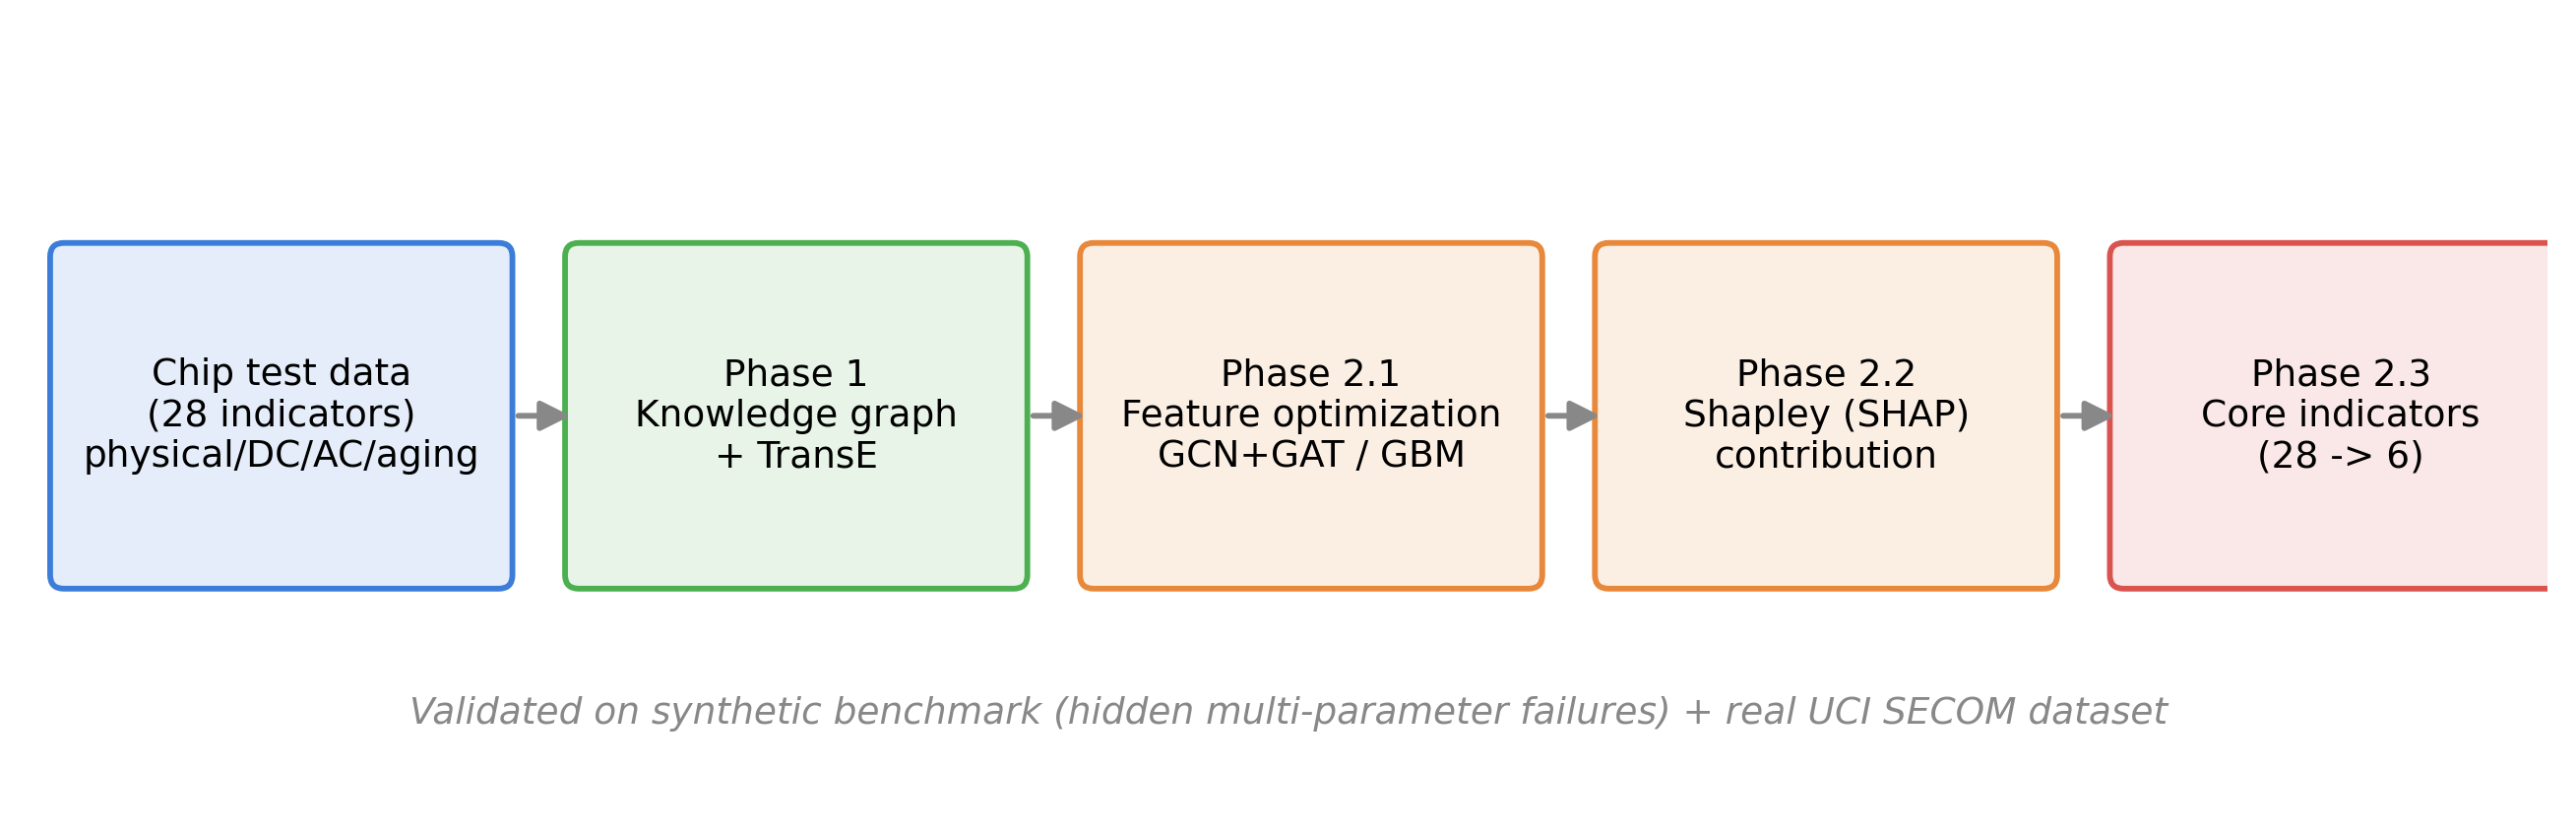
\includegraphics[width=\textwidth]{fig1_framework.png}
\caption{Overview of the proposed framework: chip test data $\rightarrow$ knowledge graph and TransE embedding (Phase~1) $\rightarrow$ feature optimization and failure identification (Phase~2.1) $\rightarrow$ Shapley contribution analysis (Phase~2.2) $\rightarrow$ core-indicator selection (Phase~2.3), validated on a synthetic benchmark and the real UCI SECOM dataset.}
\label{fig:framework}
\end{figure}

% =====================================================================
\section{Related Work}
% =====================================================================
\subsection{Circular Economy and Electronics Remanufacturing}
Systematic reviews of WEEE management consistently place reuse, refurbishment and remanufacturing high in the value-retention (``R'') hierarchy, above material recycling, because they preserve the embedded manufacturing value of components rather than recovering only raw materials~\cite{deoliveiraneto2023weee}. The same reviews observe that practice still gravitates toward end-of-pipe material recovery, partly because component-level re-qualification lacks mature, data-driven decision tools. Reliability screening of recovered components---deciding which are safe to redeploy---is exactly such a missing tool, and is the gap this work targets at the granularity of individual chips.

A closely related literature concerns recycled and counterfeit integrated circuits. Guin et al.~\cite{guin2014counterfeit} document that recycled ICs re-entering the supply chain exhibit reduced performance and shortened service lifetime, posing genuine reliability risks, and survey detection techniques ranging from on-chip aging sensors to statistical and machine-learning analyses of electrical signatures. That body of work establishes two facts that directly motivate ours: (i) the reliability of a reused chip is governed by the joint state of many electrical and physical parameters rather than any single one, and (ii) reliability degradation is detectable from test data. However, its goal is largely \emph{authentication} (is a part recycled or counterfeit?), whereas remanufacturing requires a \emph{fitness-for-reuse} decision---predicting whether a functional, salvaged chip will remain reliable. We address the latter and, in particular, the hidden-failure subproblem that single-indicator screening misses.

\subsection{Knowledge Graphs and Embeddings}
Knowledge graphs represent heterogeneous entities and their typed relations and have become a standard substrate for organizing complex engineering and scientific data~\cite{ji2022survey}. Translational embedding models, of which TransE~\cite{bordes2013translating} is the canonical example, learn low-dimensional vectors for entities and relations such that valid triples approximately satisfy a translation in embedding space; the learned geometry exposes latent associations useful for downstream mining. Random-walk embeddings such as node2vec~\cite{grover2016node2vec} provide an alternative when only structural proximity is required. We adopt a knowledge graph to organize chips, indicators and their dependencies, and use TransE to embed it and to surface indicator associations.

\subsection{Knowledge Graphs for Industrial Fault Diagnosis}
Knowledge graphs have recently been applied directly to industrial fault diagnosis. Han et al.~\cite{han2022kgevolution} construct and evolve a fault-diagnosis knowledge graph for industrial processes, while Wu et al.~\cite{wu2023mmkg} build a multimodal knowledge-graph diagnostic model to compensate for scarce fault samples. Closest to our use of graph learning, Mao et al.~\cite{mao2024gcnkg} couple a knowledge graph with a graph convolutional network for machine fault diagnosis, demonstrating that graph structure can inject relational priors into a neural classifier. These works target rotating machinery and process plants and emphasize knowledge representation and reasoning; none addresses chip-level remanufacturing or the hidden multi-parameter failure problem, and none performs SHAP-based test-indicator compression, which are the contributions of this paper.

\subsection{Graph Neural Networks}
Spectral graph convolution was made practical by fast localized filters~\cite{defferrard2016chebnet} and simplified into the widely used graph convolutional network (GCN)~\cite{kipf2017semi}, which aggregates normalized neighborhood features. Graph attention networks (GAT)~\cite{velickovic2018graph} instead learn data-dependent weights over neighbors, and inductive variants such as GraphSAGE~\cite{hamilton2017inductive} scale these ideas to large graphs; relational GCNs extend them to typed, multi-relational graphs~\cite{schlichtkrull2018rgcn}. Comprehensive surveys document their rapid adoption across domains~\cite{wu2021comprehensive}, including fault diagnosis, where sensor networks and process topologies are naturally expressed as graphs. We employ a hybrid GCN+GAT encoder over a chip-similarity graph as one of our feature-optimization models, but---consistent with the broader literature on tabular learning---we also evaluate gradient-boosted trees and report the comparison transparently.

\subsection{Tree Ensembles for Tabular Data}
Despite the prominence of deep learning, tree ensembles remain the strongest off-the-shelf models for tabular problems. Gradient boosting~\cite{friedman2001greedy} builds an additive model of shallow trees that naturally express conjunctive (AND/OR) feature interactions; scalable implementations such as XGBoost~\cite{chen2016xgboost} and LightGBM~\cite{ke2017lightgbm} are ubiquitous in applied work, and random forests~\cite{breiman2001random} provide a robust bagging alternative. Because hidden chip failures are precisely conjunctions and disjunctions of near-limit indicators, gradient boosting is a particularly apt classifier, as our experiments confirm.

\subsection{Imbalanced Learning and Feature Selection}
Chip failures are rare, so screening is an imbalanced-learning problem~\cite{he2009imbalance}; oversampling techniques such as SMOTE~\cite{chawla2002smote} are common remedies, and threshold-free metrics such as AUC are preferred to accuracy under imbalance. High-dimensional test suites also call for feature selection to remove redundant or noisy measurements~\cite{guyon2003feature}. We address imbalance through stratified cross-validation, AUC-primary reporting and validation-tuned thresholds, and we use SHAP-based ranking as an embedded feature-selection mechanism.

\subsection{Interpretability}
The Shapley value~\cite{shapley1953value} from cooperative game theory uniquely distributes a prediction among input features subject to a set of fairness axioms. SHAP~\cite{lundberg2017unified} operationalizes this for machine-learning models, TreeSHAP~\cite{lundberg2020local} computes exact Shapley values for tree ensembles efficiently, and local surrogate methods such as LIME~\cite{ribeiro2016lime} offer an alternative attribution. Beyond explanation, SHAP rankings provide a principled basis for feature (here, test-indicator) selection, which we use to compress the test suite while preserving discriminative power.

\subsection{Data-Driven Semiconductor Screening}
The UCI SECOM dataset~\cite{mccann2008secom} is a widely used real benchmark for semiconductor process fault detection, characterized by high dimensionality (590 measurements), substantial missingness and severe class imbalance (about 14:1). It has been studied extensively: Salem et al.~\cite{salem2018experimental}, for example, evaluate 288 combinations of pruning, imputation, feature selection and classification on SECOM and report ROC-AUC around the high-0.6 to 0.7 range for strong configurations, underscoring the dataset's difficulty. Most such studies treat the measurements as a flat feature vector and focus on imputation and imbalance handling. To our knowledge, the combination of a knowledge-graph representation, interaction-aware modeling, SHAP-based indicator compression, and an explicit framing around hidden multi-parameter failures for chip \emph{remanufacturing} is novel; we use SECOM as an independent, real-data check of the indicator-compression methodology and compare against reported results in Section~\ref{sec:results}.

% =====================================================================
\section{Materials and Methods}\label{sec:methods}
% =====================================================================

\subsection{Problem Formulation}
Let each chip be described by a vector of test indicators $\mathbf{x}\in\mathbb{R}^{m}$ ($m{=}28$) and a binary reliability label $y\in\{0,1\}$, where $y{=}1$ denotes a chip that is unreliable for reuse. Conventional per-indicator screening implements a decision of the form $\hat{y}=\mathbf{1}\big[\exists\, j:\, x_j\notin[\ell_j,u_j]\big]$, i.e., a chip is flagged only if some indicator $j$ falls outside its specification interval $[\ell_j,u_j]$. This rule defines an axis-aligned acceptance box and is, by design, blind to any failure whose indicators all lie inside the box. A hidden failure is precisely a chip with $y{=}1$ yet $x_j\in[\ell_j,u_j]\ \forall j$. Detecting it requires a classifier $g:\mathbb{R}^{m}\!\rightarrow[0,1]$ that depends on the \emph{joint} configuration of indicators, $g(\mathbf{x})$, rather than on per-axis tests. We pursue two coupled objectives: (i) learn such a $g$ with high ranking quality (AUC) under class imbalance; and (ii) find a small index subset $C\subseteq\{1,\dots,m\}$, $|C|\le 10$, such that a classifier restricted to the indicators in $C$ retains nearly the full discriminative power, thereby reducing measurement cost. Sections~\ref{sec:fe}--\ref{sec:shap} instantiate $g$ and the selection of $C$.

\subsection{Test Indicators}
We consider 28 chip test indicators grouped into the engineering dimensions used in industrial screening (Table~\ref{tab:indicators}): physical integrity, DC-electrical, AC-electrical/timing, functional, and reliability/aging. These cover the standard inspection performed before a chip is re-qualified and are the variables on which both the synthetic benchmark and the modeling operate.

\begin{table}[H]
\caption{The 28 test indicators by dimension.}
\label{tab:indicators}
\begin{tabularx}{\textwidth}{lX}
\toprule
\textbf{Dimension} & \textbf{Indicators}\\
\midrule
Physical (6) & pin flatness deviation, solder-pad oxidation, package scratch depth, warpage, pin coplanarity, package size deviation\\
DC-electrical (9) & VDD, IDD$_{\text{static}}$, IDD$_{\text{dynamic}}$, VOH, VOL, VIH, VIL, IIL leakage, IOL leakage\\
AC-electrical (6) & setup time, hold time, propagation delay, rise time, fall time, $F_{\max}$\\
Functional (3) & JTAG scan, boundary scan, functional test\\
Aging (4) & aging temperature, aging voltage, aging frequency, aging duration\\
\bottomrule
\end{tabularx}
\end{table}

\subsection{Synthetic Benchmark with Hidden Multi-Parameter Failures}\label{sec:data}
No public dataset pairs the full chip-level indicator set with labeled hidden-failure modes. We therefore construct a controlled synthetic benchmark of $N{=}1000$ chips with a 10\% failure rate. The construction is deliberately adversarial to per-indicator screening: hidden failures are engineered so that they cannot be separated by any single indicator threshold, while remaining physically plausible. Three design principles govern the generator.

\textbf{(1) Physical coupling.} Indicators are not sampled independently but follow engineering relationships through shared latent factors. A latent ``process-speed'' variable jointly sets the timing indicators and maximum frequency, so that dynamic power scales with frequency (empirical Pearson $r{=}0.74$ between IDD$_{\text{dynamic}}$ and $F_{\max}$), propagation delay is inversely related to $F_{\max}$ ($r{=}-0.76$), setup and hold times co-vary ($r{=}0.47$), and logic levels track the supply (VOH--VDD $r{=}0.81$). This coupling, visualized in Figure~\ref{fig:corr}, reproduces the correlation structure of real devices and is what makes single-indicator reasoning misleading.

\textbf{(2) Interaction-driven failures.} Each non-trivial failure mechanism is a \emph{conjunction} of two mildly adverse but in-specification indicators. For example, the high-side noise margin collapses only when VIH is somewhat high \emph{and} VOH is somewhat low; the timing mechanism triggers only at high frequency \emph{and} tight setup/delay; the thermal mechanism requires elevated dynamic power \emph{and} elevated warpage or leakage. A chip fails if \emph{any} mechanism triggers (a disjunction), so the failing set is the union of conjunctive corners in different indicator subspaces---a non-convex region that no single hyperplane can separate. Four modes are produced in near-balanced proportions: overt physical damage (a deliberately ``easy'', single-indicator mode), noise-margin insufficiency, thermal accumulation, and a multi-parameter combined mode.

\textbf{(3) Realism.} Aging temperature takes two stress levels (85/125\,$^\circ$C), aging drift is coupled to the latent stress, and Gaussian measurement noise is added to all indicators. By construction the three non-physical-damage modes possess no single extreme indicator; this property is verified empirically in Section~\ref{sec:results}.

\begin{figure}[H]
\centering
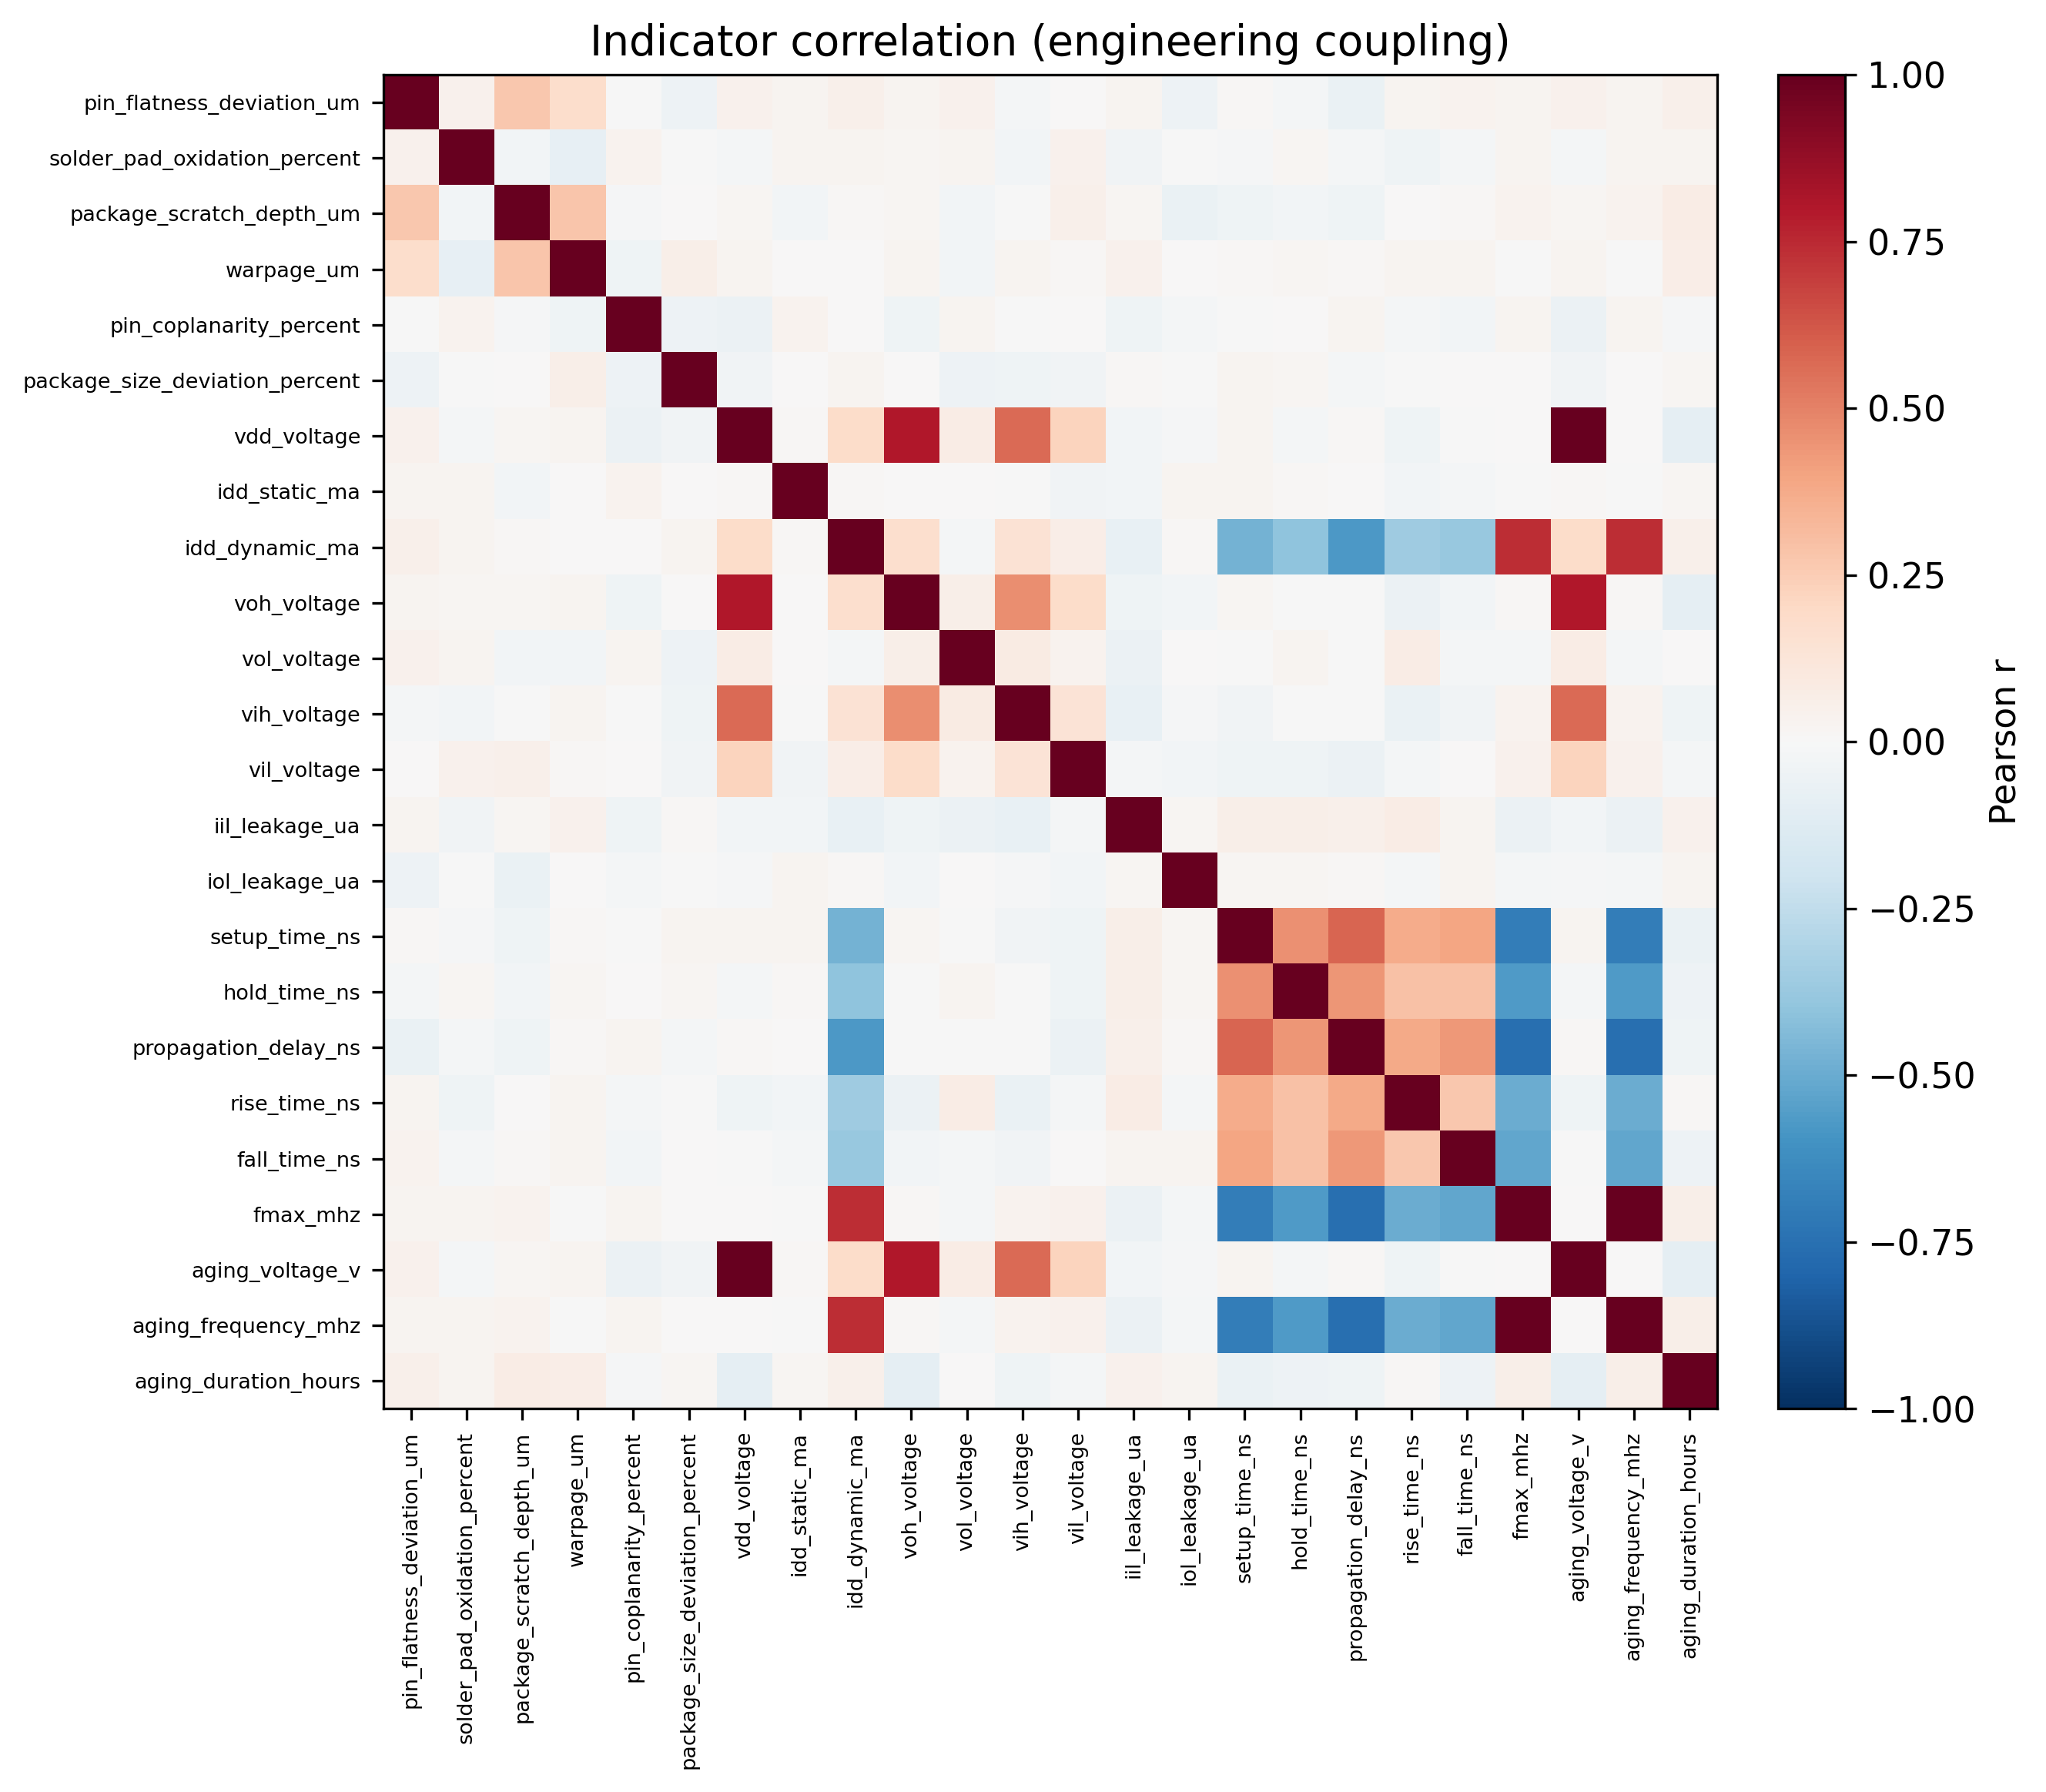
\includegraphics[width=0.72\textwidth]{fig3_correlation.png}
\caption{Pearson correlation among the continuous indicators of the synthetic benchmark, reflecting the imposed engineering coupling (e.g., IDD$_{\text{dynamic}}$--$F_{\max}$ positive, propagation delay--$F_{\max}$ negative, VOH--VDD positive).}
\label{fig:corr}
\end{figure}

\subsection{Knowledge Graph and TransE Embedding}\label{sec:kg}
We build a typed knowledge graph with six entity types (Chip, Parameter, Dimension, TestStage, FailureMode, ChipModel) and eight relation types (Table~\ref{tab:kg}). Structural edges encode domain schema: a Parameter \textsc{belongs\_to} a Dimension and is \textsc{measured\_in} a TestStage, TestStages \textsc{precede} one another, and a Chip is \textsc{of\_model} a ChipModel and \textsc{undergoes\_test} at each stage. Two relation types are data-driven and carry the analytical content: \textsc{has\_abnormal} links a chip to any indicator on which its standardized value exceeds $|z|{>}2$, and \textsc{correlates\_with} links indicator pairs whose absolute Pearson correlation is at least $0.5$, realizing basic association mining. The schema is shown in Figure~\ref{fig:kg}; the graph is materialized in a Neo4j database.

\begin{figure}[H]
\centering
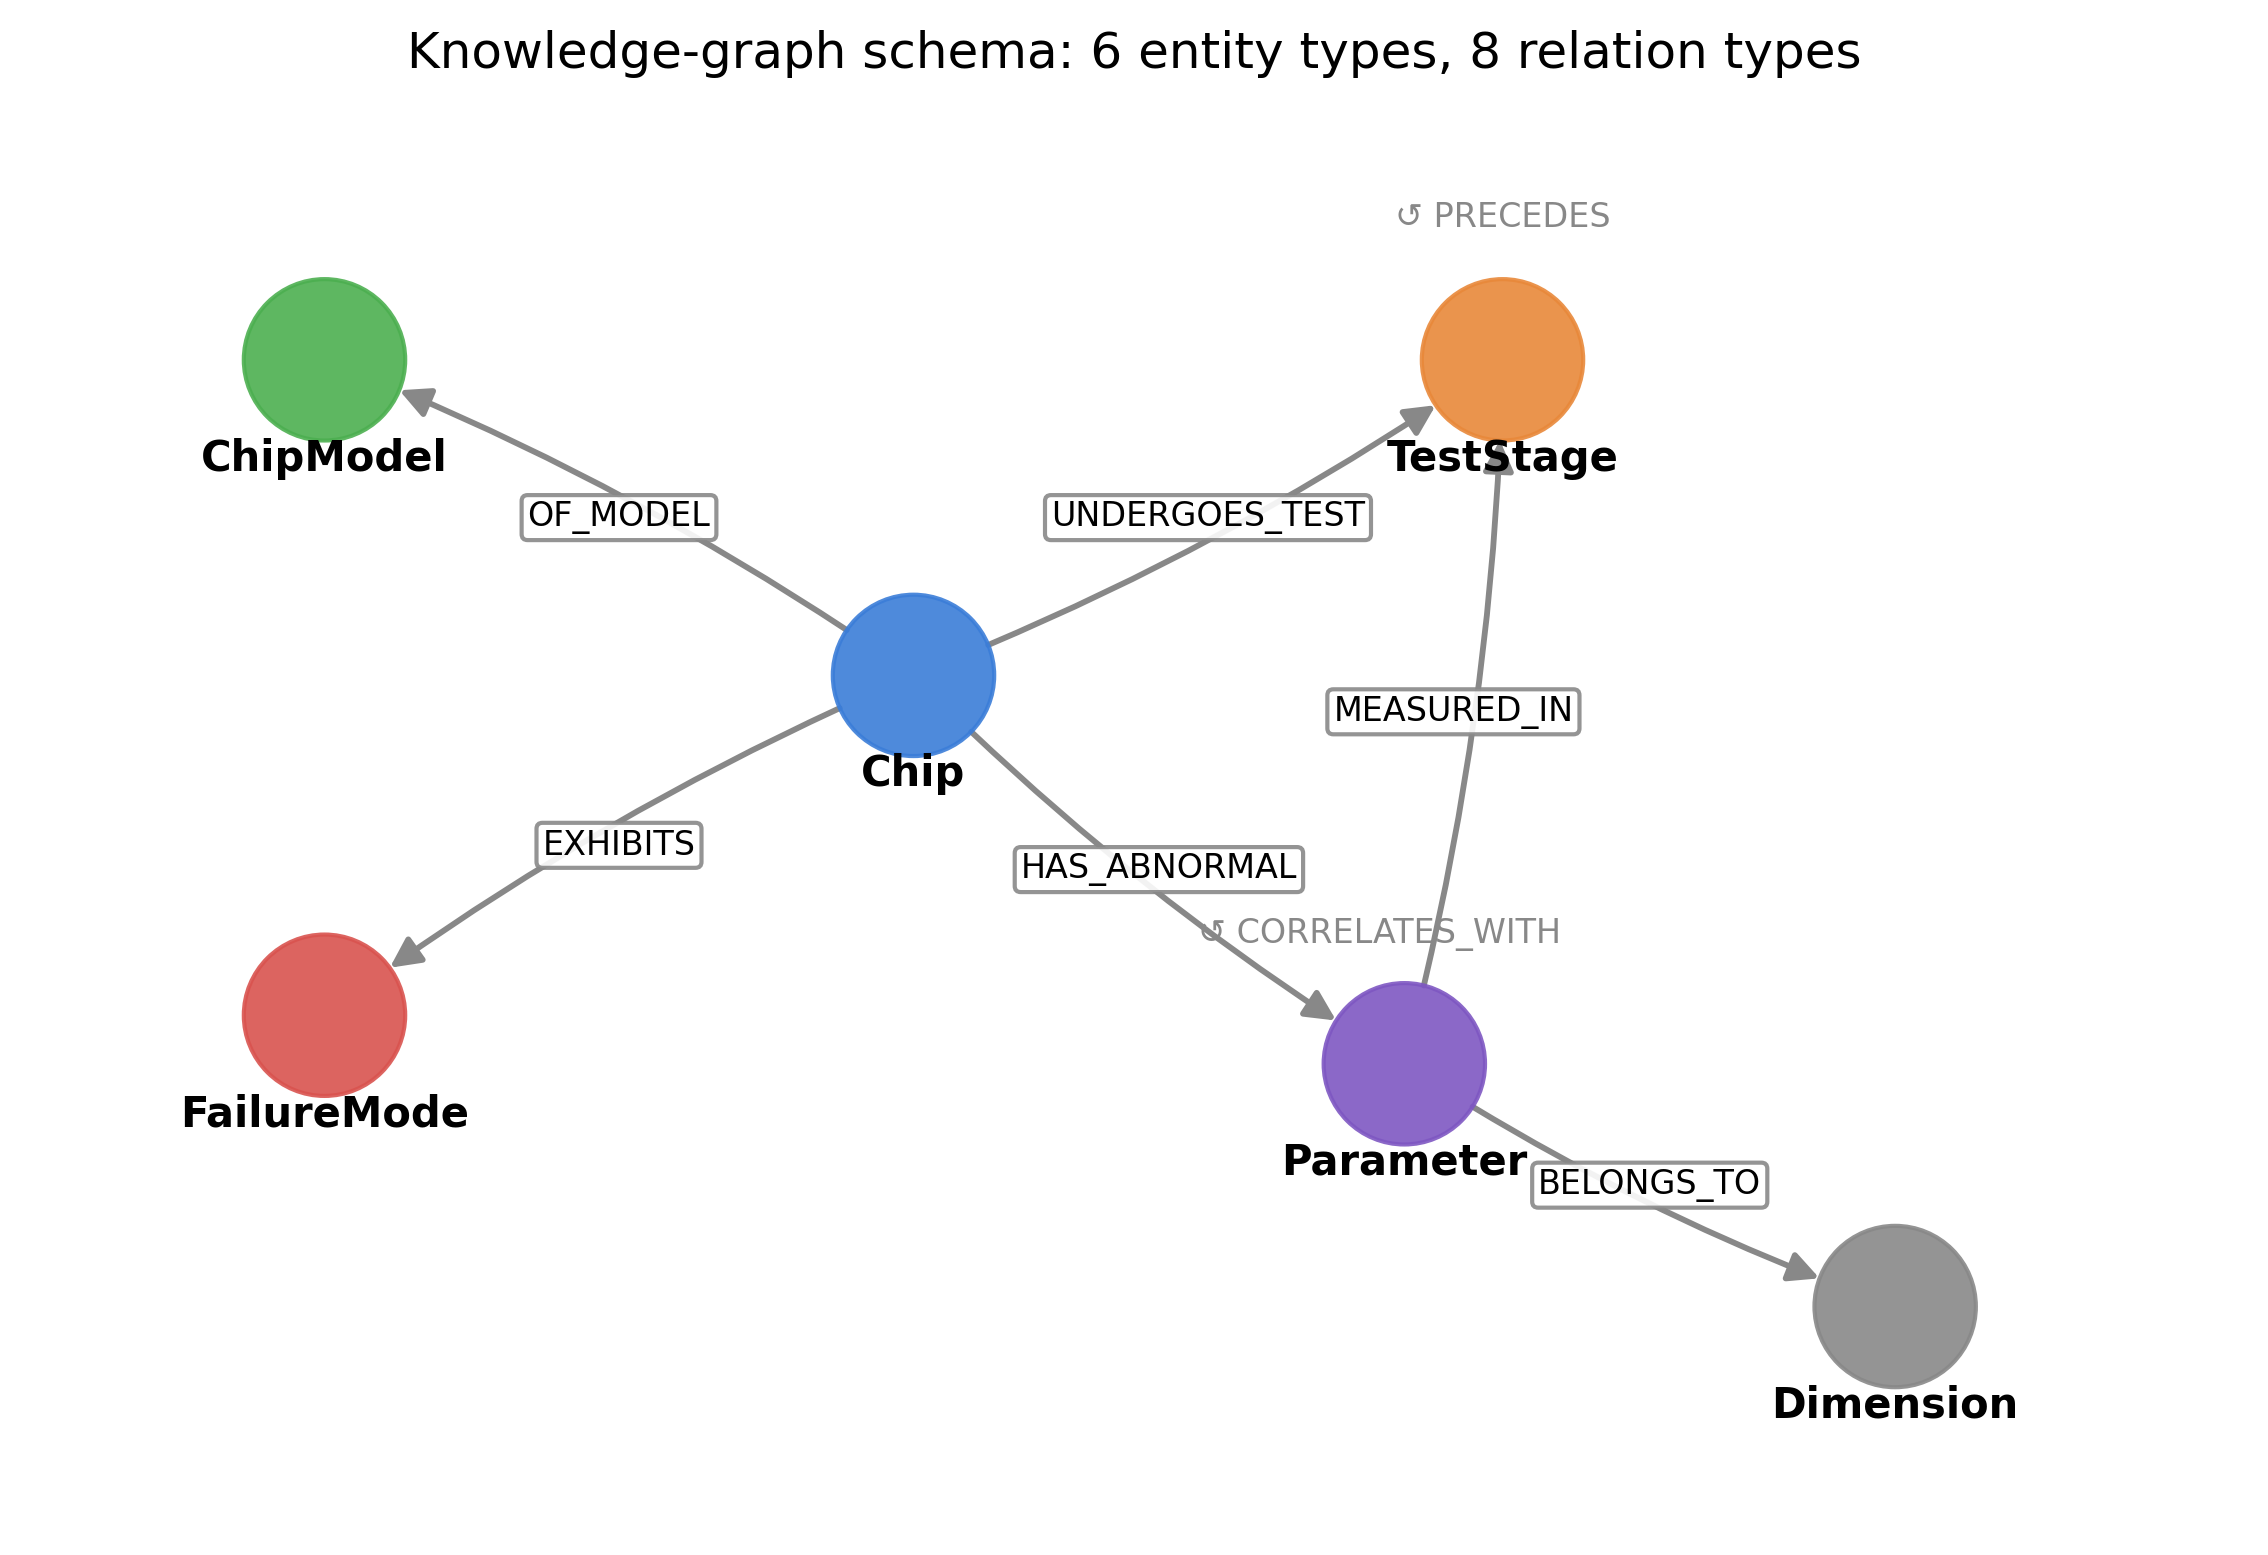
\includegraphics[width=0.8\textwidth]{fig2_kg_schema.png}
\caption{Schema of the chip-test knowledge graph: six entity types and eight relation types (two of which, \textsc{precedes} and \textsc{correlates\_with}, are self-relations).}
\label{fig:kg}
\end{figure}

We then train a TransE model~\cite{bordes2013translating} to embed entities and relations. For a triple $(h,r,t)$ with head/relation/tail embeddings $\mathbf{h},\mathbf{r},\mathbf{t}\in\mathbb{R}^{d}$ ($d{=}100$), TransE scores plausibility by the translation distance

\begin{equation}
f(h,r,t) = \lVert \mathbf{h} + \mathbf{r} - \mathbf{t} \rVert_{2},
\label{eq:transe-score}
\end{equation}

and is trained with a margin-ranking loss over positive triples $S$ and corrupted negatives $S'$ (head or tail randomly replaced):

\begin{equation}
\mathcal{L} = \sum_{(h,r,t)\in S}\ \sum_{(h',r,t')\in S'}\big[\, \gamma + f(h,r,t) - f(h',r,t') \,\big]_{+},
\label{eq:transe-loss}
\end{equation}

where $\gamma$ is the margin and $[x]_{+}=\max(0,x)$. Entity embeddings are $\ell_2$-normalized each epoch and written back to the graph as node attributes, where they serve as auxiliary relational features for downstream models.

\subsection{Feature Optimization and Failure Identification}\label{sec:fe}
\textbf{Domain feature optimization.} Beyond the 28 raw indicators we compute six interaction features that an engineer would derive directly from a datasheet: the high- and low-side noise margins ($\text{VOH}-\text{VIH}$, $\text{VIL}-\text{VOL}$), the timing slack ($1000/F_{\max}-\text{setup}-\text{delay}$), a dynamic-power proxy ($\text{IDD}_{\text{dynamic}}\cdot F_{\max}$), a thermal index, and total leakage. These make the latent failure mechanisms explicit and improve every model that consumes them.

\textbf{Hybrid GCN+GAT.} We build a $k$-nearest-neighbor chip-similarity graph ($k{=}10$) in the optimized feature space and learn node representations with a hybrid encoder that concatenates three branches: (i) a per-chip multilayer-perceptron branch that preserves each chip's own indicator combination, (ii) a GCN branch~\cite{kipf2017semi}, and (iii) a GAT branch~\cite{velickovic2018graph}. The GCN branch uses the normalized propagation rule

\begin{equation}
\mathbf{H}^{(l+1)} = \sigma\!\left(\tilde{\mathbf{D}}^{-\frac12}\,\tilde{\mathbf{A}}\,\tilde{\mathbf{D}}^{-\frac12}\,\mathbf{H}^{(l)}\mathbf{W}^{(l)}\right),
\label{eq:gcn}
\end{equation}

where $\tilde{\mathbf{A}}=\mathbf{A}+\mathbf{I}$ is the adjacency with self-loops, $\tilde{\mathbf{D}}$ its degree matrix, $\mathbf{W}^{(l)}$ the trainable weights and $\sigma(\cdot)$ a nonlinearity. The GAT branch weights neighbors $j\in\mathcal{N}(i)$ of node $i$ by learned attention

\begin{equation}
\alpha_{ij} = \frac{\exp\!\big(\mathrm{LeakyReLU}(\mathbf{a}^{\top}[\mathbf{W}\mathbf{h}_i \,\Vert\, \mathbf{W}\mathbf{h}_j])\big)}{\sum_{k\in\mathcal{N}(i)}\exp\!\big(\mathrm{LeakyReLU}(\mathbf{a}^{\top}[\mathbf{W}\mathbf{h}_i \,\Vert\, \mathbf{W}\mathbf{h}_k])\big)},\qquad
\mathbf{h}_i' = \sigma\!\Big(\sum_{j\in\mathcal{N}(i)}\alpha_{ij}\,\mathbf{W}\mathbf{h}_j\Big),
\label{eq:gat}
\end{equation}

with $\Vert$ denoting concatenation and $\mathbf{a}$ the attention vector. The three branch outputs are concatenated, projected to a 32-dimensional embedding and classified by a linear head. Because failures are scarce, we ensemble several random initializations and average their predicted probabilities to reduce variance.

\textbf{Gradient-boosted trees.} As tree ensembles excel on tabular data with conjunctive structure~\cite{friedman2001greedy,chen2016xgboost}, we also train a gradient-boosting classifier on the optimized features; this is our final classifier.

\textbf{Linear baseline.} A class-weighted logistic regression on the raw 28 indicators serves as the linear, ``no-interaction'' reference that mimics per-indicator screening with optimal linear weighting.

\subsection{Shapley Contribution and Core-Indicator Selection}\label{sec:shap}
We compute SHAP values~\cite{lundberg2017unified,lundberg2020local} for a gradient-boosting model over the 28 indicators. The Shapley value of indicator $i$ is its average marginal contribution over all feature subsets $S\subseteq F\setminus\{i\}$,

\begin{equation}
\phi_i = \sum_{S\subseteq F\setminus\{i\}} \frac{|S|!\,(|F|-|S|-1)!}{|F|!}\,\big[\,v(S\cup\{i\}) - v(S)\,\big],
\label{eq:shapley}
\end{equation}

where $F$ is the full indicator set and $v(\cdot)$ the model output for a given subset; we estimate $\phi_i$ with TreeSHAP~\cite{lundberg2020local}. Indicators are ranked by mean absolute SHAP, $\bar{\phi}_i = \frac{1}{N}\sum_{n=1}^{N}|\phi_i^{(n)}|$. We then add indicators in rank order and evaluate cross-validated performance, selecting the smallest core set (between 5 and 10 indicators) that retains at least 95\% of the full-suite AUC. Because the class distribution is imbalanced ($\sim$10\% failures), accuracy is inflated by the majority class; we therefore drive selection by AUC and report accuracy only as a secondary metric.

\subsection{Real-Data External Validation (SECOM)}
To test whether the methodology generalizes beyond our synthetic construction, we apply the same feature-selection-plus-gradient-boosting pipeline to the real UCI SECOM dataset~\cite{mccann2008secom} (1567 wafers, 590 measurements, 104 failures, $\sim$14:1 imbalance). We impute missing values with the median, drop near-constant columns (leaving 474 features), rank features by SHAP, and measure cross-validated AUC as a function of the number of selected features.

\subsection{Evaluation Protocol and Implementation}
Because failures are scarce ($\sim$100 in the synthetic set, 104 in SECOM), a single train/test split yields high-variance estimates. We therefore report \emph{5-fold stratified out-of-fold} (OOF) metrics throughout: the area under the ROC curve (AUC, threshold-free and robust to imbalance) together with accuracy, recall and F1, defined from the true/false positives and negatives ($TP,FP,TN,FN$) as

\begin{equation}
\text{Recall}=\frac{TP}{TP+FN},\quad
\text{Precision}=\frac{TP}{TP+FP},\quad
\text{F1}=\frac{2\,\text{Precision}\cdot\text{Recall}}{\text{Precision}+\text{Recall}},\quad
\text{Acc}=\frac{TP+TN}{TP+TN+FP+FN}.
\label{eq:metrics}
\end{equation}

Given the class imbalance, AUC is our primary metric; accuracy is reported only as a secondary indicator. Decision thresholds, where needed, are tuned on validation folds. Key hyperparameters are listed in Table~\ref{tab:hyper}. Models are implemented with scikit-learn~\cite{pedregosa2011scikit} (logistic regression, gradient boosting) and PyTorch (GCN+GAT); SHAP values use the TreeSHAP estimator. Random seeds are fixed and all code, data and figures are released for full reproducibility.

\begin{table}[H]
\caption{Key hyperparameters.}
\label{tab:hyper}
\begin{tabularx}{\textwidth}{lX}
\toprule
\textbf{Component} & \textbf{Settings}\\
\midrule
TransE & embedding dim 100, margin 1.0, SGD lr 0.02, 300 epochs, $\ell_2$-normalized entities\\
GCN+GAT & hidden 64, embedding 32, dropout 0.3, Adam lr 0.005, weight decay $2\times10^{-3}$, $k$-NN $k{=}10$, 4--5 ensembles\\
Gradient boosting & 100 trees, max depth 3, learning rate 0.1 (scikit-learn defaults)\\
Evaluation & 5-fold stratified out-of-fold; AUC primary; thresholds tuned on validation folds\\
\bottomrule
\end{tabularx}
\end{table}

% =====================================================================
\section{Results}\label{sec:results}
% =====================================================================

\subsection{Knowledge Graph Construction}
The constructed graph contains 1042 entities and 8179 relations across the six entity and eight relation types (Table~\ref{tab:kg}), comfortably exceeding the structural targets of $\geq$500 entities and $\geq$1000 relations set for the framework. The TransE model converges, with the margin-ranking loss decreasing monotonically from 1.013 to 0.568 over training. Standalone link-prediction quality is modest (mean reciprocal rank 0.239, Hits@10 0.456); this is expected and acceptable given the embedding's intended role as a structural/association-mining representation and auxiliary feature source rather than as a standalone classifier. The data-driven \textsc{has\_abnormal} and \textsc{correlates\_with} edges, in particular, make the indicator-association structure explicit and queryable.

\begin{table}[H]
\caption{Knowledge-graph composition (1042 entities, 8179 relations).}
\label{tab:kg}
\begin{tabularx}{\textwidth}{Xr Xr}
\toprule
\textbf{Entity type} & \textbf{Count} & \textbf{Relation type} & \textbf{Count}\\
\midrule
Chip        & 1000 & UNDERGOES\_TEST  & 5000\\
Parameter   & 25   & HAS\_ABNORMAL    & 1014\\
TestStage   & 5    & OF\_MODEL        & 1000\\
FailureMode & 5    & EXHIBITS         & 1000\\
Dimension   & 4    & BELONGS\_TO      & 25\\
ChipModel   & 3    & MEASURED\_IN     & 25\\
            &      & PRECEDES         & 4\\
            &      & CORRELATES\_WITH & $\sim$111\\
\bottomrule
\end{tabularx}
\end{table}

\subsection{Hidden Failures Are Not Visible Per Indicator}
Figure~\ref{fig:hidden} provides direct evidence that the benchmark contains genuine hidden failures. Panel~(a) plots failures in the derived noise-margin plane (high-side VOH$-$VIH against low-side VIL$-$VOL): noise-margin failures hug the low-margin edges, forming an L-shaped, non-convex region, while along either axis alone they overlap the normal population---exactly the configuration that defeats single-threshold screening. Panel~(b) reports, for each failure mode, the fraction of failed chips whose \emph{every} continuous indicator lies within $\pm2\sigma$ of the normal population. Overt physical damage is never within $\pm2\sigma$ (0\%), as intended, whereas 50\% of multi-parameter-combined failures and 24\% of noise-margin failures have no single abnormal indicator. Such chips would pass any per-indicator screen yet are genuine failures, quantifying the blind spot that motivates the framework.

\begin{figure}[H]
\centering
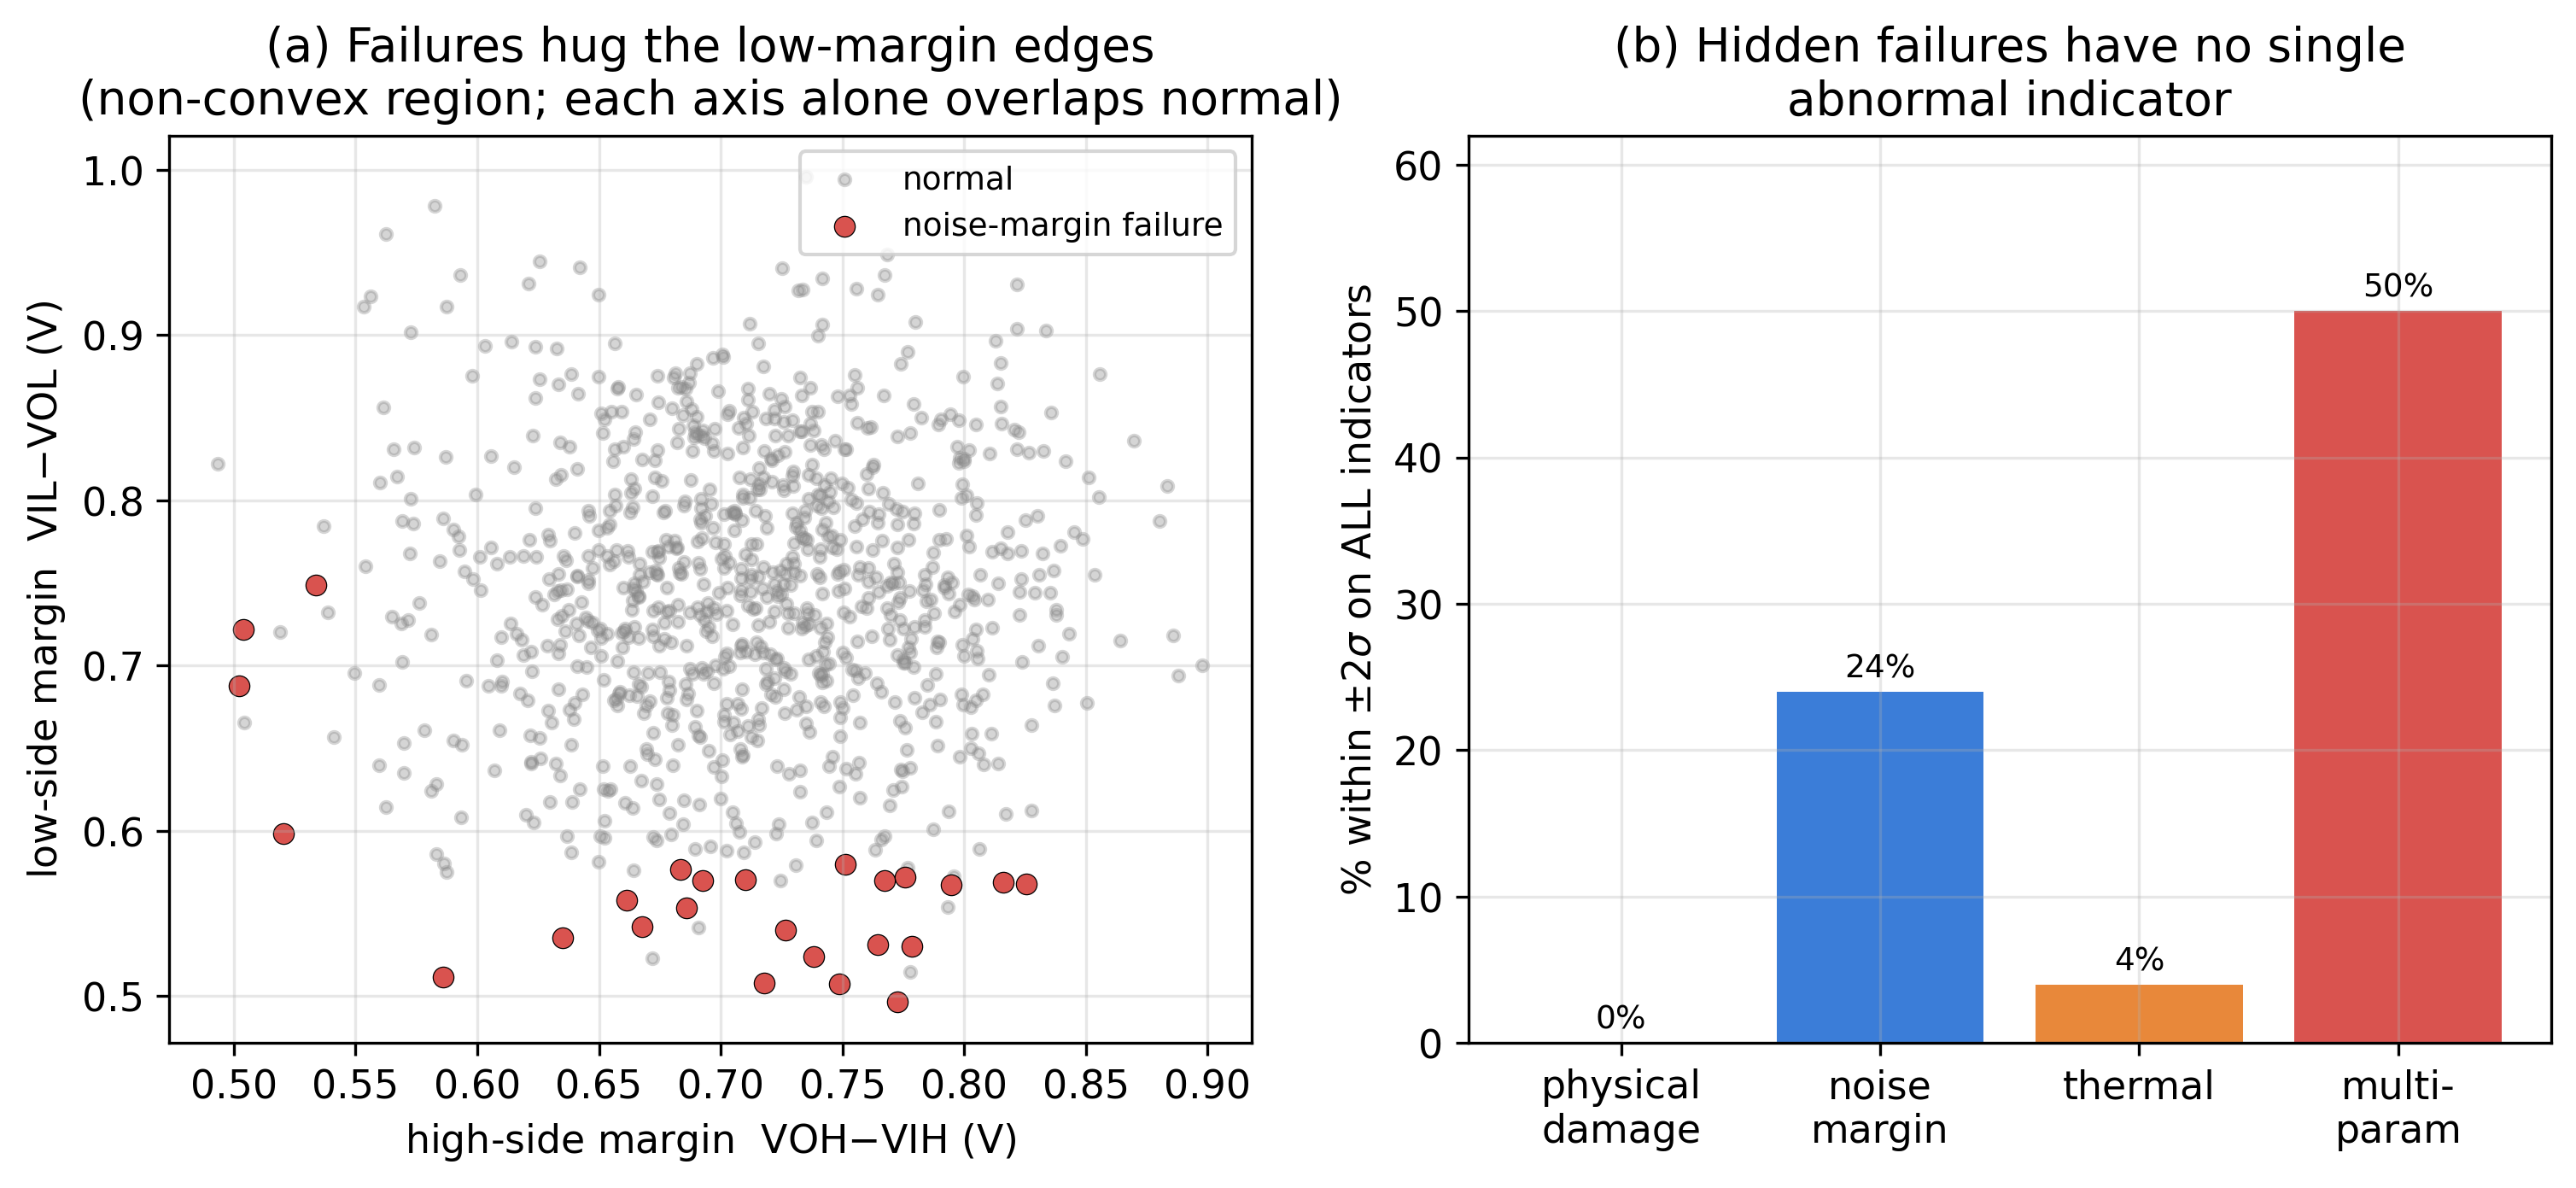
\includegraphics[width=\textwidth]{fig4_hidden_failure.png}
\caption{Evidence of hidden failures. (\textbf{a}) In the derived noise-margin plane (high-side VOH$-$VIH vs.\ low-side VIL$-$VOL), noise-margin failures hug the low-margin edges, forming a non-convex region that no single threshold separates. (\textbf{b}) Percentage of failed chips within $\pm2\sigma$ of the normal population on \emph{all} continuous indicators, by failure mode: 50\% of multi-parameter failures have no single abnormal indicator.}
\label{fig:hidden}
\end{figure}

\subsection{Linear Is Insufficient; Nonlinear Recovers the Failures}
Table~\ref{tab:models} and Figure~\ref{fig:models} compare models under 5-fold OOF evaluation. The linear baseline on raw indicators reaches only 0.845 AUC and 0.800 accuracy: optimal linear weighting of all indicators is still far from sufficient, confirming that the discriminative signal does not live in any linear combination. A gradient-boosting classifier on the same raw indicators already lifts AUC to 0.943, and on the optimized features (raw 28 plus the six interaction features) it attains 0.961 AUC, 0.940 accuracy, 0.818 recall and 0.730 F1---an AUC gain of $+0.116$ over the linear model. Domain feature optimization contributes a further $+0.018$ AUC over raw indicators. The hybrid GCN+GAT, included as the graph-representation module, reaches 0.826 AUC; consistent with the broad tabular-learning literature, tree ensembles outperform neural networks on this small, conjunctive problem, so we adopt gradient boosting as the final classifier while retaining the graph embeddings as auxiliary features. The headline practical implication is that a nonlinear, interaction-aware model raises the area under the ROC by more than eleven points over the per-indicator-style baseline at no additional measurement cost.

\begin{table}[H]
\caption{Failure-identification performance on the synthetic benchmark (5-fold OOF).}
\label{tab:models}
\begin{tabularx}{\textwidth}{lXcccc}
\toprule
\textbf{Model} & \textbf{Features} & \textbf{Accuracy} & \textbf{AUC} & \textbf{F1} & \textbf{Recall}\\
\midrule
Logistic (linear) & raw 28 & 0.800 & 0.845 & -- & --\\
GCN+GAT (ensemble) & optimized + graph & 0.803 & 0.826 & 0.398 & 0.657\\
Gradient boosting & raw 28 & -- & 0.943 & -- & --\\
\textbf{Gradient boosting (final)} & \textbf{optimized 28+6} & \textbf{0.940} & \textbf{0.961} & \textbf{0.730} & \textbf{0.818}\\
\bottomrule
\end{tabularx}
\end{table}

\begin{figure}[H]
\centering
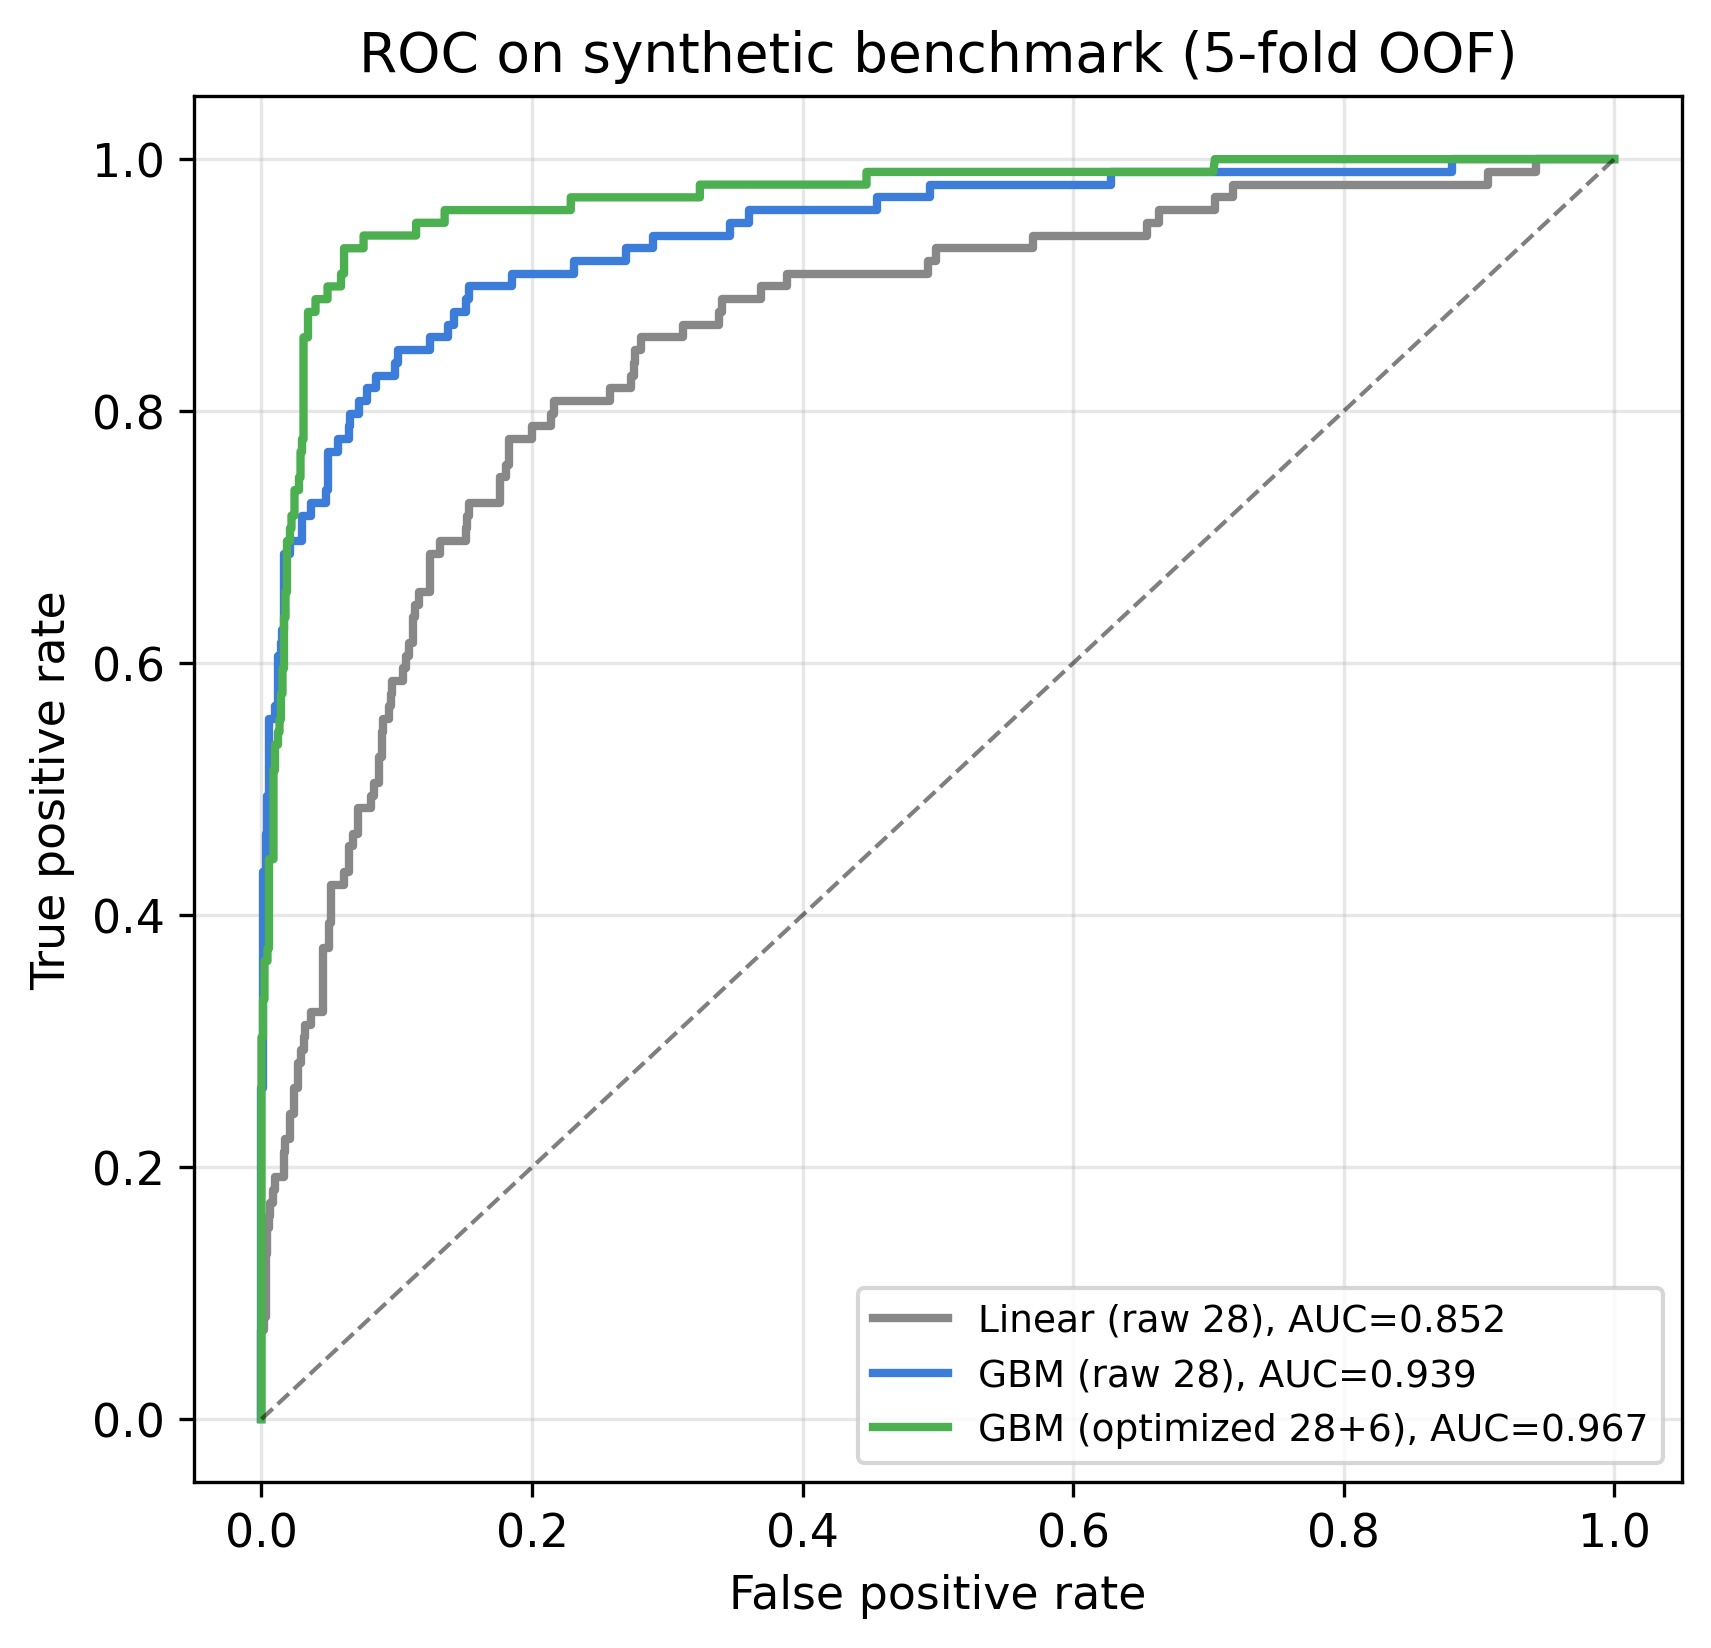
\includegraphics[width=0.6\textwidth]{fig5_roc.png}
\caption{ROC curves (5-fold OOF) on the synthetic benchmark. The nonlinear classifier on optimized features substantially outperforms the linear baseline, confirming that multi-indicator interaction governs the hidden failures.}
\label{fig:models}
\end{figure}

\subsection{Indicator Contributions and Core-Indicator Selection}
Figure~\ref{fig:shap} shows the SHAP summary for the gradient-boosting model. The most influential indicators span all three latent mechanisms: timing ($F_{\max}$, setup time, propagation delay), noise margin (VOL, VIL, VIH), and thermal (warpage, IOL leakage, IDD$_{\text{dynamic}}$). In other words, the attribution recovers exactly the indicators that, by construction, drive the failures, providing a sanity check on both the data and the method. Incremental selection (Figure~\ref{fig:selection}) shows that a 6-indicator core---$F_{\max}$, setup time, VOL, warpage, VIL, and IOL leakage---achieves 0.943 accuracy and 0.898 AUC, retaining 95.2\% of the full-suite AUC (0.943) while using only 6 of 28 indicators (Table~\ref{tab:core}). These six neatly cover the timing, noise-margin and thermal mechanisms, yielding an interpretable and substantially cheaper screening subset; reducing the test suite by more than three quarters with negligible loss of discrimination is directly actionable for a high-throughput remanufacturing line.

\begin{table}[H]
\caption{Selected 6-indicator core and the failure mechanism each represents.}
\label{tab:core}
\begin{tabularx}{\textwidth}{llX}
\toprule
\textbf{Indicator} & \textbf{Dimension} & \textbf{Mechanism}\\
\midrule
$F_{\max}$ & AC & timing (high-frequency stress)\\
setup time & AC & timing margin\\
VOL & DC & low-level noise margin\\
VIL & DC & low-level noise margin\\
warpage & physical & thermal/mechanical\\
IOL leakage & DC & thermal/leakage\\
\bottomrule
\end{tabularx}
\end{table}

\begin{figure}[H]
\centering
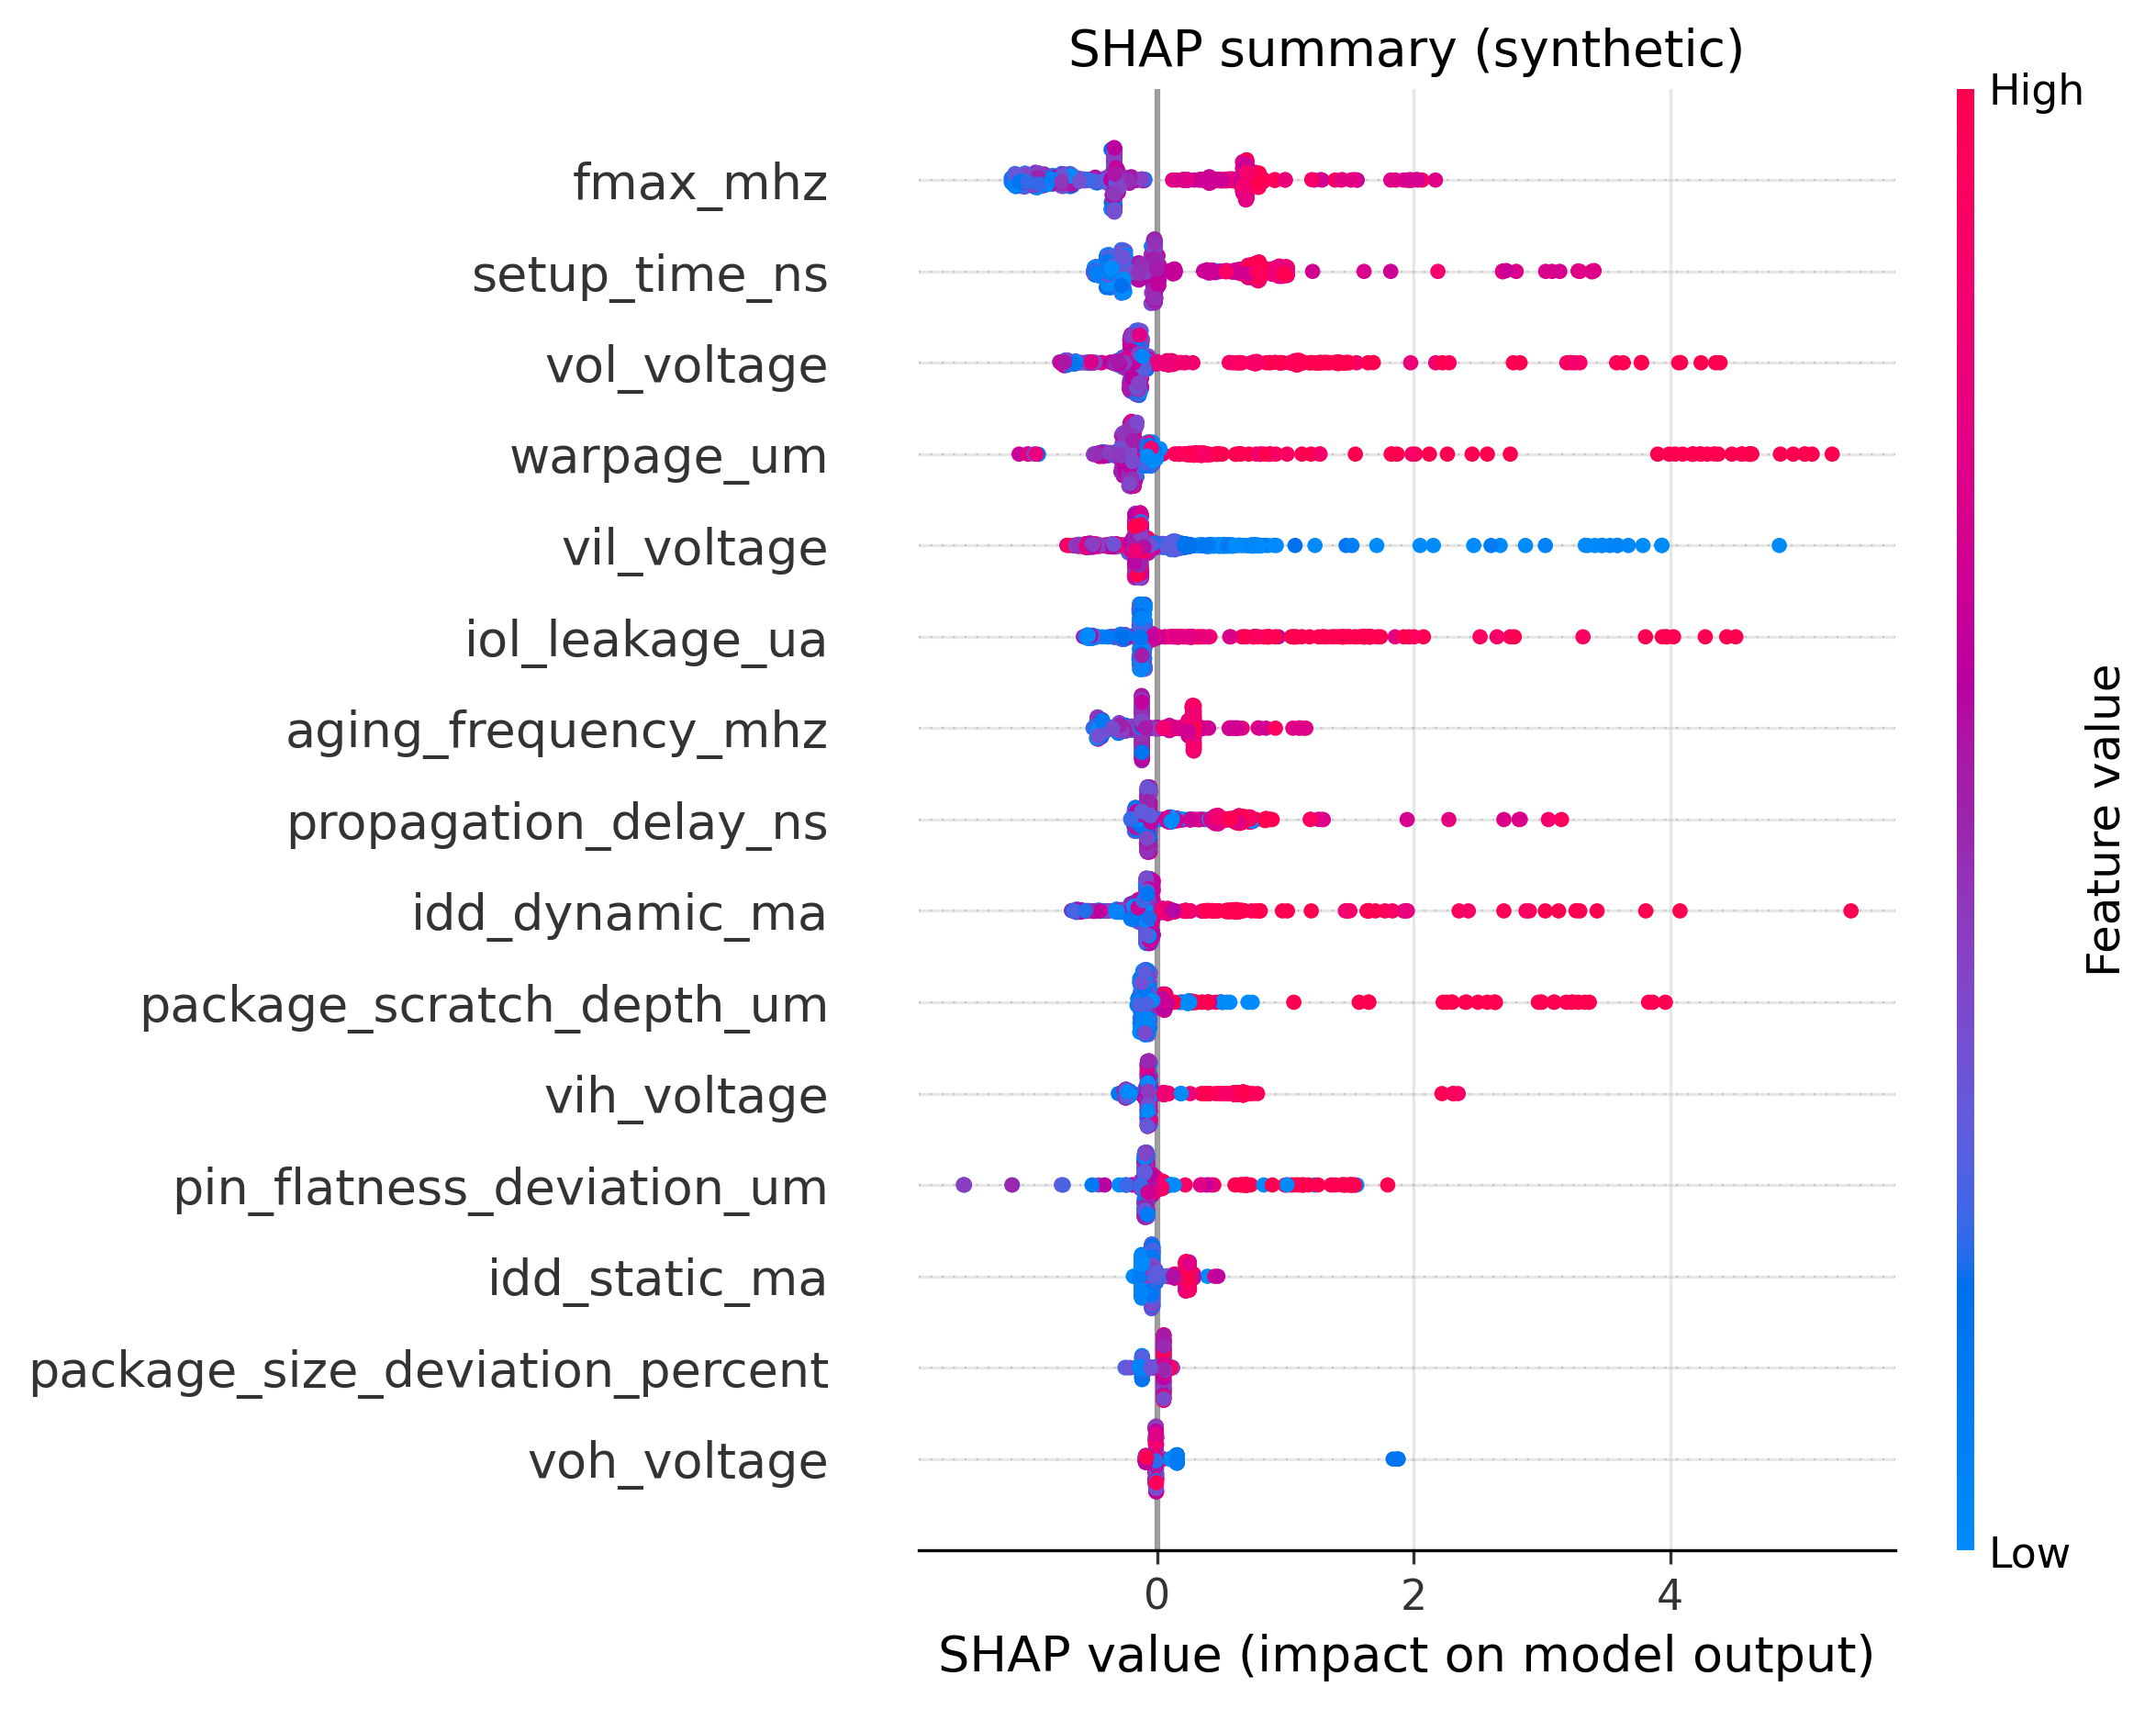
\includegraphics[width=0.85\textwidth]{fig6_shap_beeswarm.png}
\caption{SHAP summary (beeswarm) of the 15 most influential indicators on the synthetic benchmark. Each point is a chip; horizontal position is the SHAP value (impact on the failure prediction) and color encodes the indicator value (red high, blue low).}
\label{fig:shap}
\end{figure}

\begin{figure}[H]
\centering
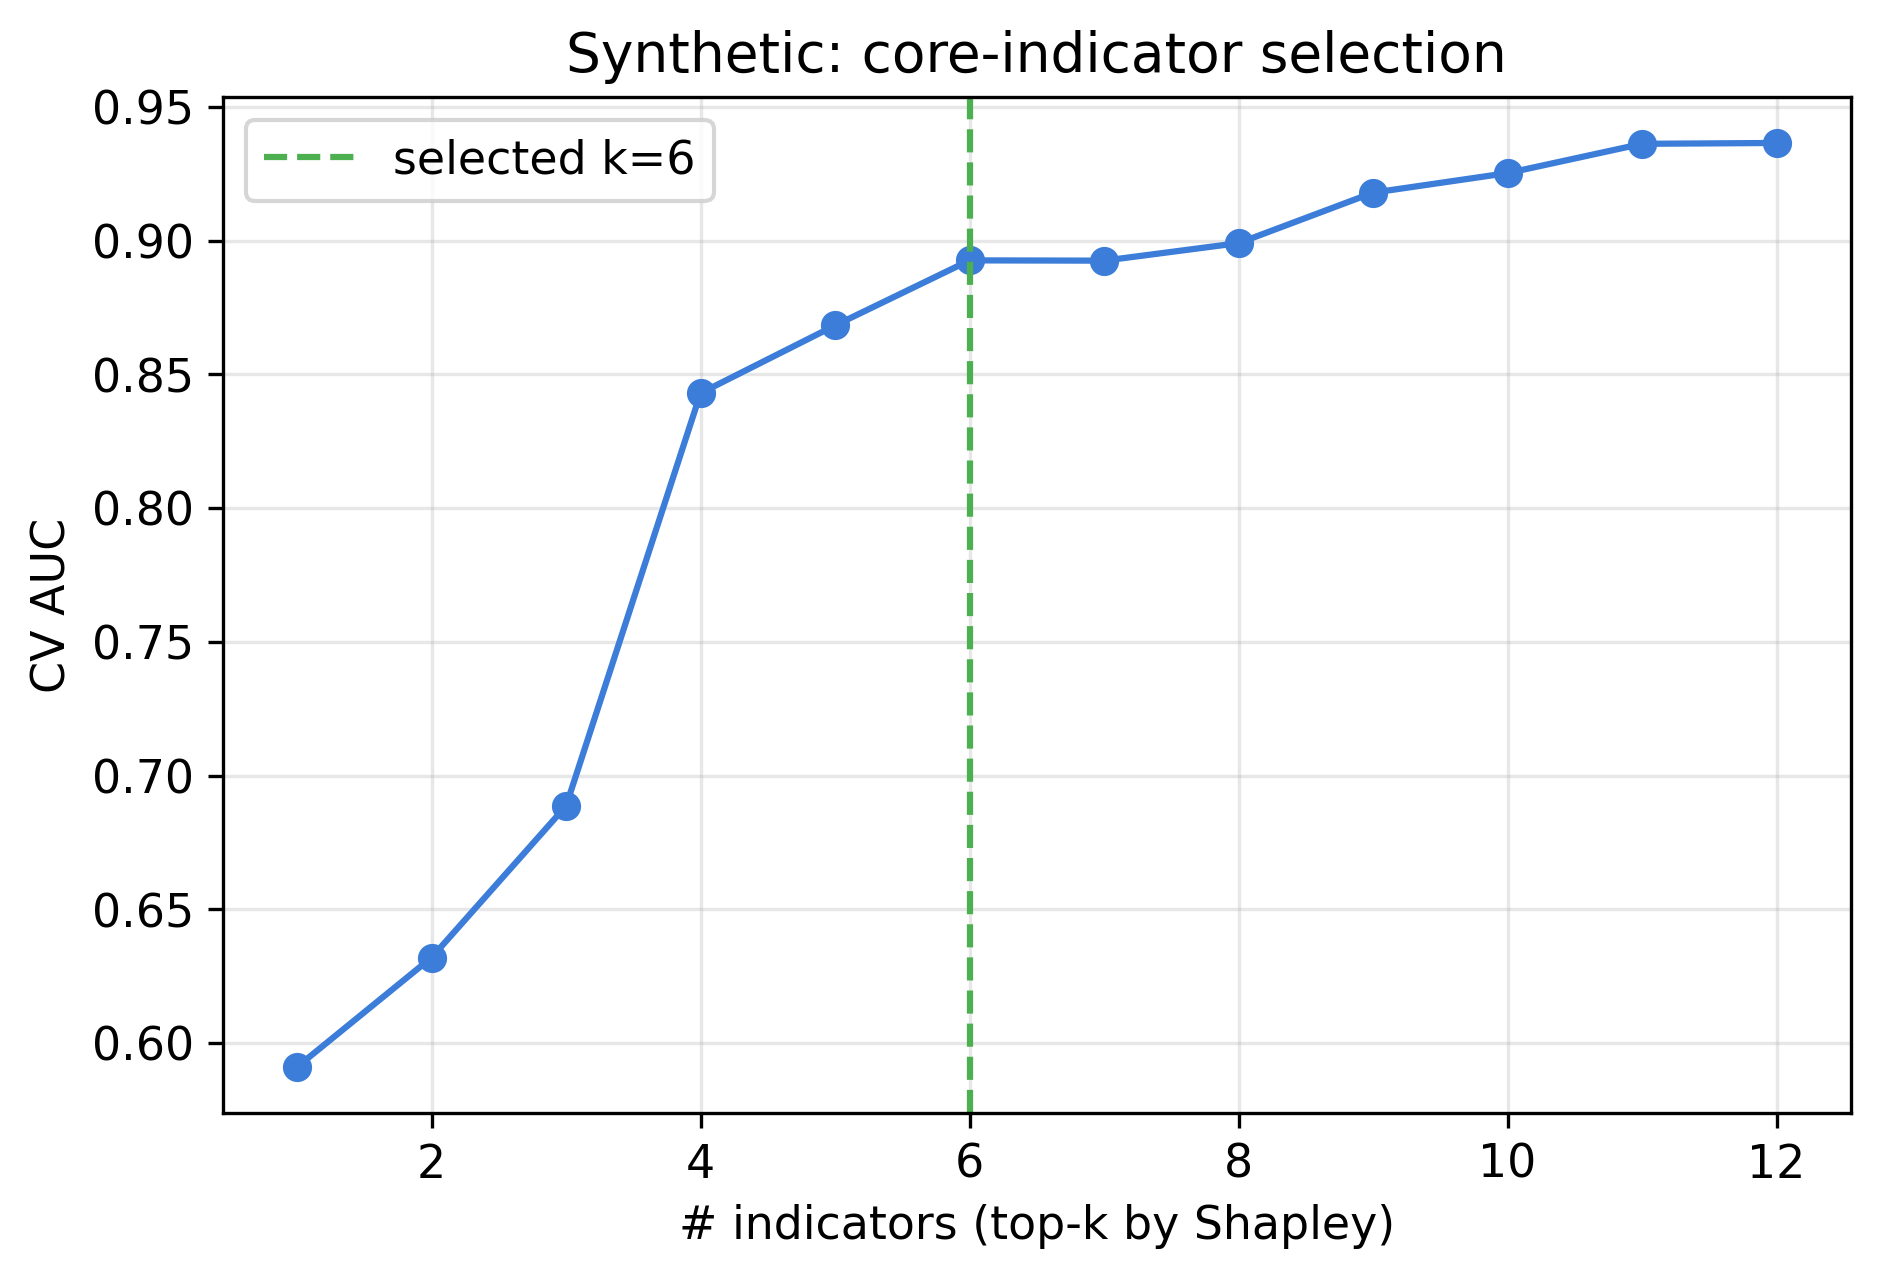
\includegraphics[width=0.7\textwidth]{fig7_core_selection.png}
\caption{Core-indicator selection on the synthetic benchmark: cross-validated AUC versus the number of top-ranked indicators; the dashed line marks the selected core size.}
\label{fig:selection}
\end{figure}

\subsection{External Validation on Real SECOM Data}
On the real SECOM dataset, a gradient-boosting classifier using all 474 retained features attains 0.687 AUC (linear: 0.655), reflecting the difficulty of this noisy, highly imbalanced benchmark (Table~\ref{tab:secom}). Applying the same SHAP-guided selection, the top 25 features raise AUC to 0.811---an improvement of $+0.124$ over using all features (Figure~\ref{fig:secom})---while as few as 5 features already match 95\% of the full-feature AUC. Thus, on genuinely real semiconductor measurements, SHAP-based selection of a compact indicator core not only compresses the measurement set but \emph{improves} discrimination by discarding noisy, redundant channels. This corroborates the synthetic-benchmark findings on independent, real data and directly mitigates the concern of evaluating solely on a self-generated dataset.

For context, our top-25 AUC of 0.811 is competitive with published SECOM results: Salem et al.~\cite{salem2018experimental}, in an extensive study of 288 pipeline combinations on the same dataset, report ROC-AUC values broadly in the high-0.6 to low-0.8 range for their strongest configurations. A strictly numeric ranking against such studies is confounded by differing preprocessing (imputation, resampling), feature counts, validation protocols and metric definitions; we therefore present this comparison as indicative rather than as a state-of-the-art claim. The salient, protocol-independent observation is internal and therefore fair: under one fixed pipeline, replacing all 474 features by a SHAP-selected subset raises AUC by $+0.124$, demonstrating the value of interaction-aware indicator selection on real data.

\begin{table}[H]
\caption{Results on the real UCI SECOM dataset (5-fold OOF).}
\label{tab:secom}
\begin{tabularx}{\textwidth}{Xccc}
\toprule
\textbf{Configuration} & \textbf{\#Features} & \textbf{AUC} & \textbf{Accuracy}\\
\midrule
Logistic (all features) & 474 & 0.655 & 0.909\\
Gradient boosting (all features) & 474 & 0.687 & 0.934\\
\textbf{Gradient boosting (SHAP top-25)} & \textbf{25} & \textbf{0.811} & --\\
Gradient boosting (SHAP top-5) & 5 & 0.683 & --\\
\bottomrule
\end{tabularx}
\end{table}

\begin{figure}[H]
\centering
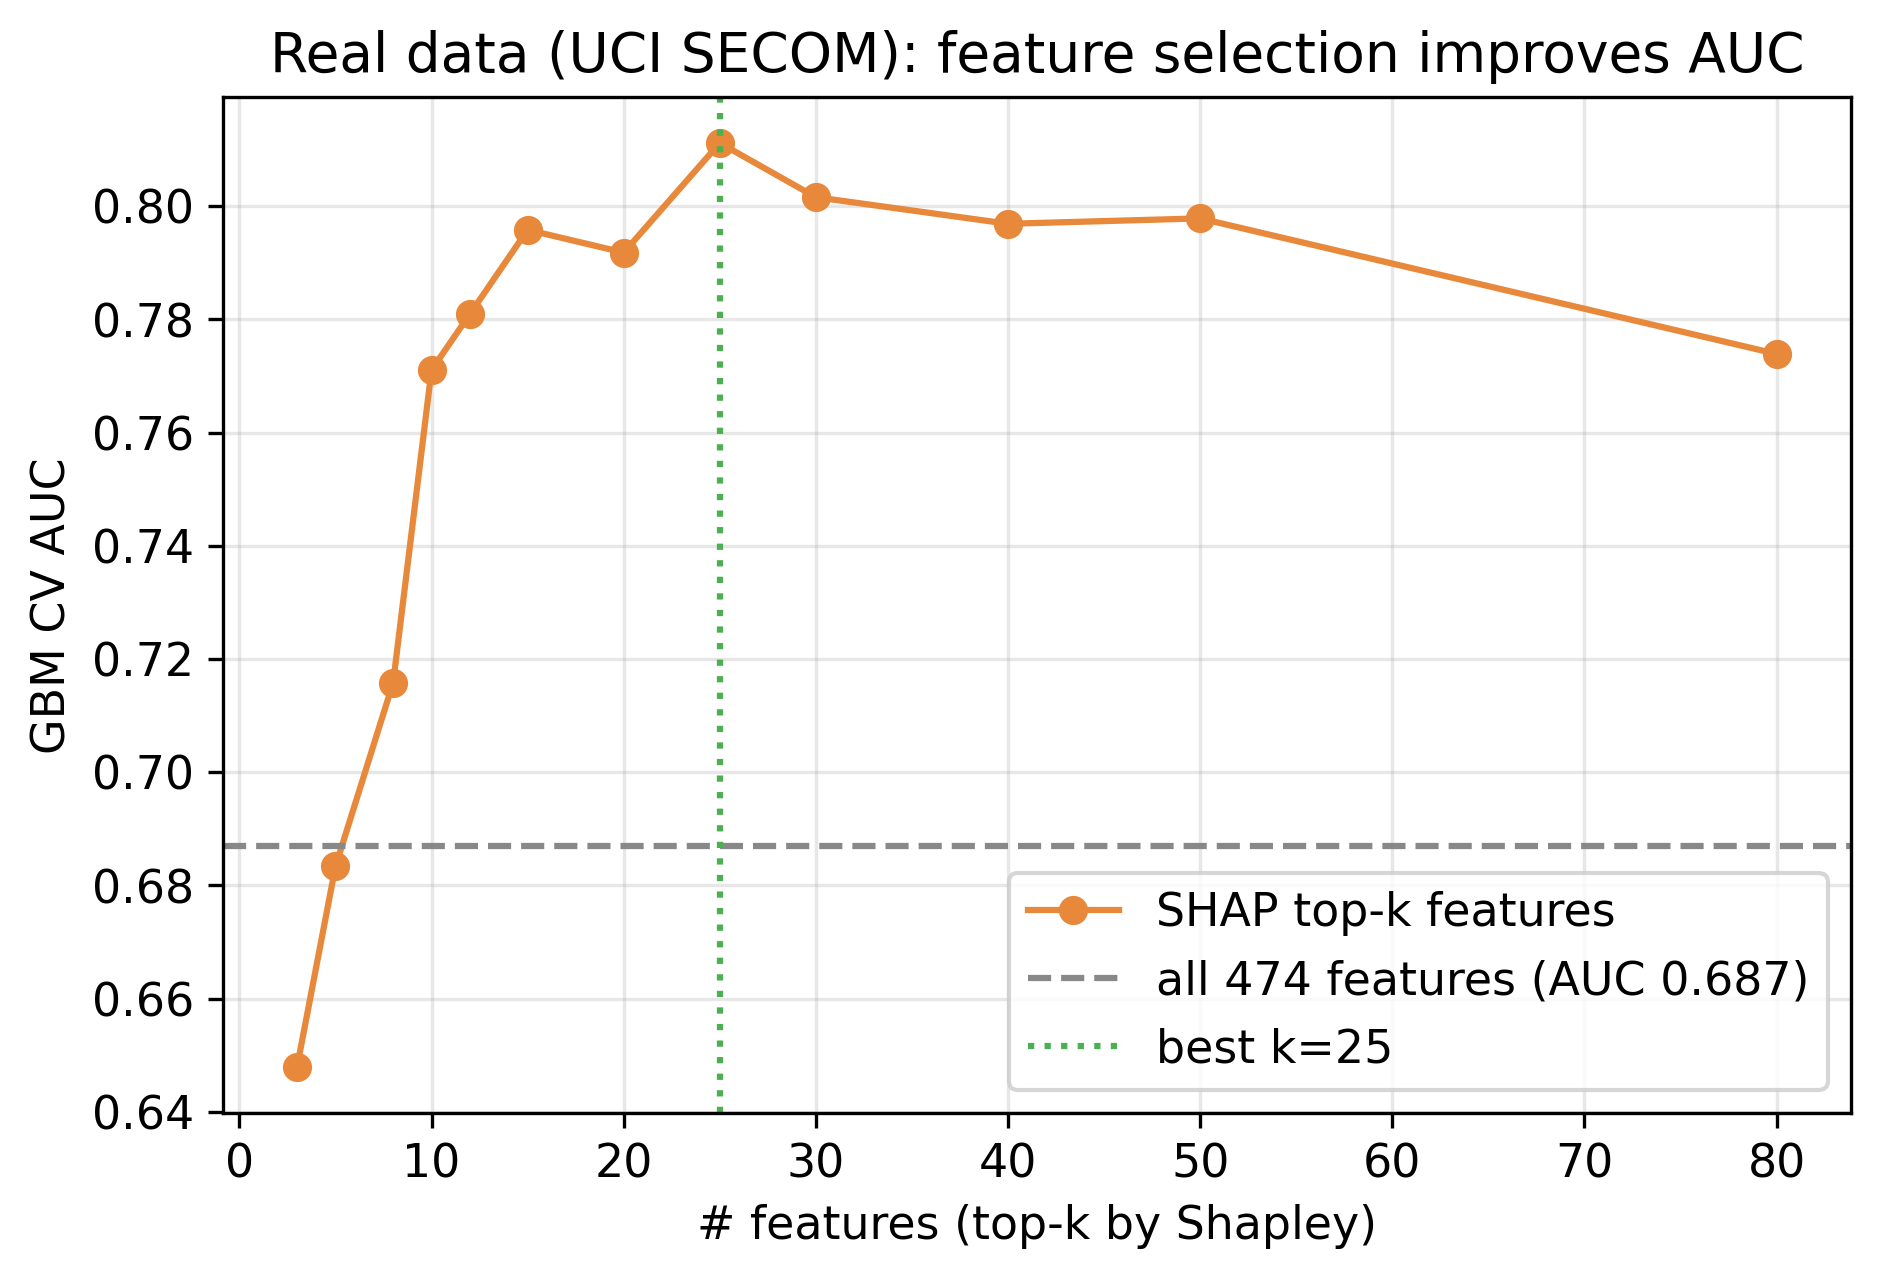
\includegraphics[width=0.7\textwidth]{fig8_secom_validation.png}
\caption{External validation on the real UCI SECOM dataset: cross-validated GBM AUC versus the number of SHAP-selected features. Selecting $\sim$25 features outperforms using all 474.}
\label{fig:secom}
\end{figure}

\subsection{Ablation Study}
To isolate the contribution of each component, Table~\ref{tab:ablation} reports a controlled ablation under the identical 5-fold OOF protocol, toggling the model family (linear vs.\ gradient boosting vs.\ GCN+GAT), the feature set (raw 28, the 6 interaction features alone, or both), and the indicator subset (full vs.\ SHAP core 6).

\begin{table}[H]
\caption{Ablation on the synthetic benchmark (5-fold OOF AUC). Each axis is toggled while holding the others fixed.}
\label{tab:ablation}
\begin{tabularx}{\textwidth}{Xlc}
\toprule
\textbf{Model} & \textbf{Features / indicators} & \textbf{AUC}\\
\midrule
Linear (logistic) & raw 28 & 0.845\\
Linear (logistic) & raw 28 + 6 interaction & 0.846\\
GCN+GAT (ensemble) & raw 28 + 6 interaction (+ graph) & 0.826\\
Gradient boosting & 6 interaction features only & 0.841\\
Gradient boosting & SHAP core 6 indicators & 0.898\\
Gradient boosting & raw 28 & 0.943\\
\textbf{Gradient boosting} & \textbf{raw 28 + 6 interaction (full model)} & \textbf{0.961}\\
\bottomrule
\end{tabularx}
\end{table}

Four observations follow. \emph{(i) Model family dominates:} replacing the linear classifier by gradient boosting on identical raw inputs raises AUC from 0.845 to 0.943 ($+0.098$), the single largest jump, isolating the value of nonlinear interaction modeling. \emph{(ii) Interaction features help trees, not linear models:} the six engineered margins lift the gradient-boosting model from 0.943 to 0.961 ($+0.018$) yet barely move the linear model (0.845$\rightarrow$0.846), precisely because the failures are disjunctive/non-convex and a linear decision surface cannot exploit the margins even when they are provided explicitly. \emph{(iii) Compression is nearly free:} the SHAP core of 6 indicators reaches 0.898, retaining 95\% of the full-model AUC with about one-fifth of the indicators, and even 6 engineered features alone (0.841) already match the full linear baseline. \emph{(iv) Graph is auxiliary:} the GCN+GAT (0.826) does not exceed the tree models, confirming that the chip-similarity graph and TransE embeddings serve best as representation and association-mining tools rather than as the predictive backbone. On real SECOM data the feature-count sweep (Figure~\ref{fig:secom}) further shows that performance is non-monotone in the number of indicators---AUC peaks near 25 features and then declines---so the optimum is a compact core rather than the full suite. Overall, the framework's gains stem mainly from interaction-aware classification and SHAP-guided compression, and are robust to the exact size of the selected core within a broad plateau.

% =====================================================================
\section{Discussion}
% =====================================================================
Three findings stand out. First, on data with genuine hidden-failure structure, single-indicator and linear screening are demonstrably insufficient: the AUC gap of $+0.116$ between the linear baseline and the nonlinear classifier on the synthetic benchmark, together with the $+0.124$ improvement from feature selection on real SECOM data, both show that the discriminative signal lives in nonlinear combinations of indicators. This provides quantitative support for the central premise that chip re-qualification should be modeled jointly across indicators rather than indicator by indicator, and explains why purely threshold-based screening lets hidden failures through.

Second, interpretable attribution makes the resulting models actionable. SHAP recovers the physically meaningful drivers of failure---timing, noise-margin and thermal indicators---and enables an aggressive reduction of the test suite (28$\rightarrow$6 on the synthetic benchmark, with a comparable compression on SECOM) at negligible or even positive impact on discrimination. For remanufacturing lines, where test time dominates per-unit cost, such a compact, well-understood core directly reduces screening cost and provides a natural foundation for adaptive, sequential test ordering.

Third, model choice should follow the data rather than fashion. Although graph neural networks are attractive for relational data, on this tabular, conjunctive task gradient-boosted trees were consistently stronger; we therefore use the graph components for representation and association mining and the tree ensemble for classification, and we report this trade-off transparently. We regard such honesty about negative or mixed results as essential to a trustworthy engineering methodology.

\textbf{Practical implications for remanufacturing lines.} In a high-throughput remanufacturing setting, end-to-end test time per chip is the dominant cost driver, and each indicator corresponds to a measurement that consumes instrument time and fixturing. A screening model that retains discrimination while using six of twenty-eight indicators therefore translates fairly directly into reduced test time and higher line throughput, provided the omitted measurements are not required for other purposes. Equally important, the per-prediction SHAP attribution gives operators a human-readable reason for each rejection (e.g., a collapsed noise margin or a thermal--timing interaction), which supports engineering trust, root-cause triage and audit. The compact core is also a natural starting point for sequential or adaptive testing, in which inexpensive, high-information indicators are measured first and further testing is conditioned on intermediate results---an avenue we leave to future work but which the present indicator ranking directly enables.

\textbf{Generalization and transferability.} Two pieces of evidence speak to generalization. First, the synthetic results are obtained under stratified cross-validation with held-out folds, so they reflect generalization to unseen chips rather than memorization. Second, and more importantly, the indicator-compression methodology transfers to the real SECOM dataset, which differs from our synthetic benchmark in domain (wafer fabrication vs.\ chip screening), dimensionality (590 vs.\ 28), missingness and imbalance ratio; that the same SHAP-then-boosting recipe improves AUC there as well suggests the approach is not an artifact of our data-generating assumptions. We nonetheless caution that absolute performance numbers are dataset-specific and that transfer to a particular remanufacturing line will require recalibration on that line's data.

\textbf{Threats to validity and limitations.} The primary limitation is data. The controlled benchmark is synthetic; although its parameter ranges and failure mechanisms are grounded in device-physics reasoning and its conclusions are corroborated by the real SECOM results, it is not a substitute for labeled field data from an operating remanufacturing line, and synthetic constructions inevitably embed the designer's assumptions. The SECOM dataset, while real, originates from wafer fabrication rather than retired-chip screening, so it validates the feature-selection and interaction-modeling methodology rather than the full chip-remanufacturing scenario. The TransE embedding's standalone link-prediction quality is modest, and the graph module underperforms the tree classifier. Finally, accuracy figures are inflated by class imbalance and should be read alongside AUC and recall. We have mitigated these concerns through cross-validated evaluation, a linear and a tree baseline, an explicit hidden-failure analysis, and independent real-data validation, but they bound the strength of the present claims.

\textbf{Future work.} We plan to (i) acquire real retired-chip test and field-return data to replace or augment the synthetic benchmark, (ii) couple the selected core indicators with reinforcement-learning-based adaptive test ordering to cut screening time while maintaining accuracy, and (iii) extend the framework from binary failure detection to compatibility and risk prediction for redeployment scenarios, closing the loop toward a deployable remanufacturing decision system.

% =====================================================================
\section{Conclusions}
% =====================================================================
We presented a knowledge-graph-guided framework for detecting hidden multi-parameter failures and selecting a compact core of test indicators for retired-chip remanufacturing. On a controlled benchmark engineered to contain failures invisible to per-indicator screening, nonlinear models on optimized features reached 0.961 AUC and 0.940 accuracy versus 0.845 for a linear baseline, and SHAP-based selection compressed 28 indicators to 6 while retaining 95\% of the AUC. The methodology generalized to the real UCI SECOM dataset, where SHAP-guided feature selection improved AUC from 0.687 to 0.811. Together these results show that interaction-aware, interpretable modeling can both expose failures that conventional screening misses and reduce the number of measurements required to find them, offering a practical decision aid for circular-economy chip reuse. Integrating real field data and adaptive test ordering is the main avenue toward deployment.

\vspace{6pt}

% --- MDPI back matter (fill in before submission) ---
\authorcontributions{Conceptualization, methodology, software, validation, writing---all authors. All authors have read and agreed to the published version of the manuscript.}
\funding{This research received no external funding.}
\dataavailability{The synthetic data generator, all experiment code and figures are available in the project repository. The SECOM dataset is publicly available at the UCI Machine Learning Repository, \url{https://doi.org/10.24432/C54305}.}
\conflictsofinterest{The authors declare no conflict of interest.}

% References are managed via BibTeX (refs.bib) with the MDPI style (Definitions/mdpi.bst).
\bibliography{refs}

\end{document}
